\documentclass[conf]{new-aiaa}
%\documentclass[journal]{new-aiaa} for journal papers
\usepackage[utf8]{inputenc}

\usepackage{graphicx}
\usepackage{amsmath}
\usepackage[version=4]{mhchem}
\usepackage{siunitx}
\usepackage{longtable,tabularx}
\usepackage{fixme}
\setlength\LTleft{0pt}
\hypersetup{
  colorlinks=true
}

% Setup fixme env for collaborative notes
\fxsetup{status=draft, layout=inline, theme=color}

\title{Computation and comparison of the stable Northeastern US marine boundary layer}

\author{Lawrence C. Cheung\footnote{Principal member of technical staff, Thermal/Fluid Science \& Engineering, AIAA member}}
\affil{Sandia National Laboratories, Livermore, CA 94550}

\author{
  Shreyas Ananthan\footnote{SOME JOB TITLE, AIAA Member},
  Michael J. Brazell\footnote{Researcher III, High-Performance Algorithms and Complex Fluids, AIAA Member},
  Ganesh Vijayakumar\footnote{Researcher III, Mechanical Engineering, AIAA Member}, and
}
\affil{National Renewable Energy Laboratory, Golden CO 80401}

\author{Nathaniel B. deVelder\footnote{Postdoctoral appointee, Wind
    Energy Technologies Department, AIAA member} and Alan
  S. Hsieh.\footnote{Postdoctoral appointee, Wind Energy Technologies
    Department, AIAA member}} \affil{Sandia National Laboratories,
  Albuquerque, NM 87185}

\begin{document}

\maketitle

\begin{abstract}
Put abstract here
\end{abstract}

\section{Nomenclature}

{\renewcommand\arraystretch{1.0}
\noindent\begin{longtable*}{@{}l @{\quad=\quad} l@{}}
$\alpha$  & Wind shear exponent  \\
$f$       & Frequency \\
$L$       & Turbulent integral length scale \\
$u_\tau$   & Friction velocity    \\
$R_{ij}$   & Two point correlation tensor \\
$TI$      & Turbulence intensity \\
$TKE$     & Turbulent kinetic energy 
\end{longtable*}}

\section{Introduction}
\fxnote{Update this introduction.}

\lettrine{T}he planned installation of several offshore wind energy
plants in the United States has highlighted the need to properly
understand the wind resource and atmospheric characteristics of the US
Atlantic Coast.  Several atmospheric phenomena particular to this
region, such as coastal low-level jets or seasonal Nor’easters, have
the potential to substantially impact the operation and power
production of offshore wind plants.  Of particular interest to the
current study is the atmospheric stability of the marine boundary
layer in the Northeastern US.

Atmospheric stability plays a large role in determining the power
production of wind plants because it directly affects the vertical
distribution of momentum and turbulent energy in the atmospheric
boundary layer (ABL).  The differences between the stable, neutral, or
unstable stratified ABL can lead to large changes in wind speed or
turbulence profiles, and ultimately change the operation of wind
turbines.  Atmospheric stability may also play a role in the formation
of low-level jets \cite{nunalee2014mesoscale} and cause increased
fatigue loads on offshore wind turbines.

Several recent measurement campaigns have provided data to understand
the ABL and wind characteristics for potential offshore wind farms in
the Northeastern US.  Pichugina et al. \cite{pichugina2017properties}
measured the wind profiles and vertical shear profiles in the Gulf of
Maine using a ship-borne lidar approach.  Analysis of measured data
sets from Nantucket Sound by Archer et
al. \cite{archer2016predominance} showed a predominance of low-shear,
unstable conditions at the site.  However, strong seasonal variations
and stratification changes due to diurnal variation were also
observed.

In addition to these measurements, large eddy simulations (LES) have
also been used to study ABL stability characteristics.  Recent work by
Kaul et al. \cite{kaul2020large} has shown that LES computations using
Nalu-Wind can capture the neutrally and convectively unstable onshore
ABL.  Previous simulations by Cheung et al. \cite{cheung2020large}
successfully replicated the unstable and neutral ABL corresponding to
the Cape Wind meteorological tower measurements
\cite{archer2016predominance} and showed the effects of surface
heating on atmospheric stratification.  Additional LES computations
\cite{sullivan2016turbulent} have also previously explored stable
conditions of onshore boundary layers, such as the GABLS1 boundary
layer \cite{beare2006intercomparison}.  However, a complete comparison
including offshore stable ABL conditions has yet to be completed.

\subsection{Prevous work}

\fxnote{Mention study by \cite{wurps2020grid}.  Nate's piece goes here.}

\subsection{Outline}

The current paper is organized as follows.

%%%%%%%%%%%%%%%%%%%%%%%%%%
%% SECTION 2: METHODOLOGY
%%%%%%%%%%%%%%%%%%%%%%%%%%
\section{Methodology}
Write something about what we're comparing with, the codes we're
using, and how we set up the simulations.

\subsection{Measured offshore conditions}
% \fxnote{Lawrence write this part}

Following the work of Cheung et al \cite{cheung2020large}, we use
measurements of the offshore coastal marine boundary layer, collected
by the Cape Wind meteorological tower in Nantucket Sound, as the basis
for this computational study.  The Cape Wind platform collected wind
measurements at 20m, 41m, and 60m above the mean water level, along
with temperature and barometric measurements from the years 2003-2011.
From the observations, Archer et al.\cite{archer2016predominance}
found that the marine boundary layer is predominantly unstable, with
61\% of conditions classified as unstable, versus 21\% neutral and
18\% stable.  The stratification of the marine boundary layer, as
determined by the Obukhov length, also had a large impact on the wind
speed profile, with flatter, non-logarithmic profiles seen during
unstable conditions.

From the measured distribution of atmospheric stabilities, turbulent
kinetic energies (TKE), and wind speeds from the Cape Wind platform at
z=20m, a stable set of conditions were chosen as targets for this
computational study.  A summary of the conditions for all stability
classes is given table \ref{tab:CapeWindMeasurements}. In this work we
focus on the three stable atmospheric conditions at wind speeds of
5m/s, 10m/s, and 15m/s, while the neutral and unstable conditions
where studied in previous work \cite{cheung2020large}.

To maintain consistency with the measured data, the turbulence
intensity (TI) is calculated using the TKE as
\begin{equation}
  \textrm{TI} =
  \frac{\sqrt{\frac{2}{3}\times\textrm{TKE}}}{\overline{U}_{horiz}} =
  \frac{\sqrt{\frac{1}{3}\left( \overline{u'u' + v'v' + w'w'}
      \right)}}{\overline{U}_{horiz}}
\end{equation}
The averaged wind speeds were enforced at the measurement height of
20m, and the applied wind directions were consistent with the
predominant stable direction of 225 degrees southwest.

\begin{table}
\caption{\label{tab:CapeWindMeasurements} Measured conditions at Cape
  Wind.  The stable atmospheric conditions used in this study are
  highlighted in bold below.} \centering
\begin{tabular}{cccc}
  \hline
  Stability    & Wind speed [m/s] & Wind dir [deg] & Turbulence intensity \\
  \hline
  Neutral      & 5                & 225            & 0.055           \\
  Neutral      & 10               & 225            & 0.055           \\
  Neutral      & 15               & 225            & 0.065           \\
  Unstable     & 5                & 315            & 0.080           \\
  Unstable     & 10               & 315            & 0.075           \\
  Unstable     & 15               & 315            & 0.090           \\
  \bf{Stable}  & \bf{5}           & \bf{225}       & \bf{0.045}      \\
  \bf{Stable}  & \bf{10}          & \bf{225}       & \bf{0.050}      \\
  \bf{Stable}  & \bf{15}          & \bf{225}       & \bf{0.060}      \\
\hline
\end{tabular}
\end{table}


\subsection{Computational methodology}
Provide a general description of the LES codes that we use.

Large Eddy Simulations (LES) of the stable atmopsheric conditions described in
Table~\ref{tab:CapeWindMeasurements} are performed using the open-source,
ExaWind simulation environment\footnote{\url{https://github.com/exawind}}.
ExaWind is a suite of high-fidelity modeling tools for analyzing complex
microscale atmospheric boundary layer flows and wind farm flows. The present
study uses two different incompressible computational fluid dynamic solvers
available within the ExaWind suite --
Nalu-Wind~\footnote{\url{https://github.com/exawind/nalu-wind}} and
AMR-Wind~\footnote{\url{https://github.com/exawind/amr-wind}}. This section
briefly describes the incompressible Navier-Stokes equations solved in the
solvers, the specifics of the turbulence model and the wall shear stress
formulation used to model the terrain, and the details of the numerical
discretization of the two equations in the two codes.

\subsection{LES formulation}

\subsubsection{Governing equations}
Both CFD codes solve the incompressible form of Navier-Stokes equations with
appropriate models for turbulence closure. Equation~\ref{eqn:ns-les} shows the
continuity and momentum equations with all the terms necessary to model the
atmospheric boundary layer problem. Term $\mathbf{I}$ represents the pressure
gradient forces as a deviation from hydrostatic and horizontal mean gradient,
term $\mathbf{II}$ represents the contribution from viscous and sub-filter scale
stresses, term $\mathbf{III}$ represents the contribution from Coriolis forces
due to earth's rotation, term $\mathbf{IV}$ represents the effects of buoyancy,
and term $\mathbf{V}$ represents source terms necessary to drive the flow to a
desired horizontal mean velocity at prescribed heights.

\begin{align}
  \frac{\partial \bar{\rho}} {\partial t} + \frac{\partial \bar{\rho} \widetilde{u_j}}{\partial x_j} & = 0, \nonumber\\
  \frac{\partial}{\partial t} \left(\bar{\rho}\, \widetilde{u}_i\right) +
  \frac{\partial}{\partial x_j} \left( \bar{\rho}\, \widetilde{u}_i \widetilde{u}_j \right) &=
  - \underbrace{\frac{\partial p'}{\partial x_j} \delta_{ij}}_\mathbf{I}
  - \underbrace{\frac{\partial \tau_{ij}}{\partial x_j}}_\mathbf{II}
  - \underbrace{2\bar{\rho}\,\epsilon_{ijk}\,\Omega_j\widetilde{u_k}}_\mathbf{III}
  + \underbrace{\left(\rho - \rho_\circ \right) g_i}_\mathbf{IV}
  + \underbrace{S^{u}_{i}}_\mathbf{V} \label{eqn:ns-les}
\end{align}

For the simulations presented in this paper, the buoyancy term ($\mathbf{IV}$)
is approximated using the Bousinessq model. The Bousinessq model ignores the
effect of density gradients on inertia while retaining its effects on buoyancy.
The density fluctuations governing the buoyancy effects are approximated as

\begin{align*}
  \frac{\rho}{\rho_\circ} \approx 1 - \beta \left( \theta - \theta_\circ \right)
\end{align*}
This leads to a forcing term that depends on potential temperature ($\theta$),
the reference density $\rho_\circ = \bar{\rho}$, and thermal expansion
coefficient $\beta \approx 1 / \theta_\circ$ as
\begin{align}
  \left(\rho - \rho_\circ \right) g_i = -\rho_\circ\, \beta\, g_i \left( \theta - \theta_\circ \right)
\end{align}

For ABL problems, the conservation of energy equation is usually written in
terms of potential temperature as shown in Eq.~\ref{eqn:pot-temp-les}.
\begin{align}
  \frac{\partial}{\partial t} \left(\bar{\rho}\, \widetilde{\theta}\right) +
  \frac{\partial}{\partial x_j} \left(\bar{\rho}\, \widetilde{u}_j \widetilde{\theta} \right) = - \frac{\partial}{\partial x_j} \hat{q}_j \label{eqn:pot-temp-les}
\end{align}
Under the assumption of ideal gas conditions and constant specific heat capacity
$c_p$, the gradients in potential temperature are proportional to the gradients
in absolute temperature, i.e.,
\begin{align*}
   \left[ \frac{\partial T}{\partial t}, \frac{\partial T}{\partial x}, \frac{\partial T}{\partial y} \right] =
   \left( \frac{\bar{p}}{p_\circ} \right)^{\left(\frac{R}{c_p}\right)} \left[ \frac{\partial \theta}{\partial t}, \frac{\partial \theta}{\partial x}, \frac{\partial \theta}{\partial y} \right]
\end{align*}
Furthermore, ignoring the pressure and viscous work terms in
Eq.~\ref{eqn:pot-temp-les}, for incompressible flows, it can be shown that
solving the enthalpy equation is equivalent to solving the potential temperature
equation. The enthalpy equation solved in Nalu-Wind for wind energy problems is
shown below
\begin{align}
  \frac{\partial}{\partial t} \left(\bar{\rho}\, \widetilde{h}\right) +
  \frac{\partial}{\partial x_j} \left(\bar{\rho}\, \widetilde{u}_j \widetilde{h} \right) = - \frac{\partial}{\partial x_j} q_j \label{eqn:enthalpy-les}
\end{align}
It is noted here that the terms $\hat{q}_j$ (Eq.~\ref{eqn:pot-temp-les}) and
$q_j$ (Eq.~\ref{eqn:enthalpy-les}) are not equivalent and must be scaled
appropriately. User can still provide the appropriate initial and boundary
conditions in terms of potential temperature field. Under these assumptions and
conditions, the resulting solution can then be interpreted as the variation of
potential temperature field in the computational domain.

The subgrid-scale kinetic energy ($k$) one-equation turbulence model
(Eq.~\ref{eqn:ksgs-les}), based on Moeng~\cite{Moeng1984}, is used for
LES turbulence closure.

\begin{align}
  \frac{\partial}{\partial t}\left(\bar{\rho} k \right) + \frac{\partial}{\partial x_j} \bar{\rho} k \widetilde{u_j} &= \frac{\partial}{\partial x_j} \left (2 \nu_t \frac{\partial k}{\partial x_j} \right) - 2 \nu_t \widetilde{S_{ij}} \widetilde{S_{ij}} + \frac{g}{\theta_\circ} \tau_{\theta_i} - C_{\epsilon} \frac{k^{3/2}}{l} \label{eqn:ksgs-les}
\end{align}
where
\begin{align*}
  C_\epsilon &= 0.93 & \nu_t &= C_\epsilon l \sqrt{k} \\
  \tau_{\theta i} &= - 2\ \frac{\nu_t}{\mathrm{Pr}_t}\ \frac{\partial \widetilde{\theta}}{\partial x_i} & \mathrm{Pr}_t &= \left( 1 + \frac{2l}{\Delta} \right)^{-1} \\
\end{align*}
The choice of the length scale ($l$) depends on whether the stratification is positive
or negative, based on the recommendation by Moeng~\cite{Moeng1984}, and is given
by
\begin{align*}
  l =
  \begin{cases}
    \Delta = \sqrt[3]{\Delta_x \Delta_y \Delta_z}, & \frac{\partial \widetilde{\theta}}{\partial z} < 0 \\
    0.76\, \sqrt{k}\, \frac{g}{\theta_\circ}\, \left( \frac{\partial \widetilde{\theta}}{\partial z}\right)^{-1/2}, &  \frac{\partial \widetilde{\theta}}{\partial z} > 0 \\
  \end{cases}
\end{align*}

\begin{comment}
  \fxnote{Shreyas write this part.  Currently placeholder equations below.}\\

  The low-Mach number equations:
  \begin{align}
    \frac{\partial \rho} {\partial t} + \frac{\partial \rho u_j}{\partial x_j} & = 0, \\
    \frac{\partial \rho u_i}{\partial t} + \frac{\partial \rho u_j u_i}{\partial x_j}
    + \frac{\partial P}{\partial x_i} & = \frac{\partial \tau_{ij}}{\partial x_j}
                                        + \left( \rho - \rho_{\circ} \right) g_i, \\
    \frac{\partial \rho h}{\partial t} + \frac{\partial \rho u_j h}{\partial x_j} & =
                                                                                    - \frac{\partial q_j}{\partial x_j} + \frac{\partial P_{th}}{\partial t},
  \end{align}
\end{comment}

\subsubsection{\label{sec:wallmodelBC}Lower wall model BC}
\fxnote{Ganesh write this part}\\
What we implemented in terms of the lower boundary condition.

\subsubsection{Nalu-Wind}

Nalu-Wind~\cite{SpragueAVR2020} is an open-source, wind-focused fork of the Nalu CFD
code~\cite{Domino:2015}. The codebase heavily leverages the open-source Trilinos
suite of numerical libraries~\cite{Heroux:2003}. Nalu-Wind uses an
unstructured-grid, node-centered, finite-volume formulation for solving the incompressible
Navier-Stokes equations. Two spatial discretization approaches are supported
within the codebase -- the edge-based scheme and control-volume finite-element
scheme. The edge-based scheme, used in the present study, is similar to the
classical cell-centered finite volume formulation formulated on a dual volume
surrounding the nodes of the mesh. The governing equations are discretized in
time using a split-operator approach. Implicit backward difference formula
(BDF2) timestepping algorithm with an approximate pressure projection
scheme~\cite{Moen-Domino:2003} is used to advance the equations in time.
Multiple Picard-style outer-loop iterations are employed within each timestep
to minimize the errors introduced from split-operator approximations. Nalu-Wind
comes equipped with a suite of Reynolds-Averaged Navier-Stokes (RANS), LES, and
Detached Eddy Simulation (DES) turbulence models to resolve the disparate
spatial and temporal scales encountered when modeling wind plant flows.

Nalu-Wind heavily utilizes the Sierra Toolkit (STK) library~\cite{Edwards:2010}
for managing the unstructured mesh data structures. The linear systems resulting
from the discretized equations are solved using solvers available within the
Belos and MueLu libraries within Trilinos. The momentum and scalar transport
equations are solved using GMRES iterative solver with symmetric Gauss-Seidel
(SGS) preconditioners. The elliptic pressure-Poisson equation is solved using
GMRES solvers with a smoothed-aggregated algebraic multigrid preconditioner. The
reader is referred to Sprague et al.~\cite{SpragueAVR2020} and
Domino~\cite{Domino:2015} more more details.

While the primary objective of Nalu-Wind within the ExaWind simulation suite is
to support blade-resolved simulations of wind turbines, it comes equipped
with all the physics models necessary for modeling atmospheric boundary flows.
In the present work, the prognostic equation for temperature is solved using the
enthalpy equation (Eq.~\ref{eqn:enthalpy-les}). The prognostic one-equation,
subgrid-scale kinetic energy equation (Eq.~\ref{eqn:ksgs-les}) is used for LES
turbulence closure. Two Picard iterations were employed within each timestep to
minimize splitting errors and recover second-order accuracy in time.

\subsubsection{AMR-Wind}

\fxnote{Do we want a github link reference for amr-wind? exawind?}\\

As part of a suite of physics codes within the open-source project called ExaWind, 
AMR-Wind enables more efficient and scalable simulations of wind power plants. 
This is because it is built on top of the AMReX software framework which contains 
all of the functionality needed to develop massively parallel, block-structured 
adaptive mesh refinement (AMR) applications \cite{AMReX_JOSS}.
Since AMR-Wind is limited to Cartesian block-structured grids it is specialized
to handle atmospheric boundary layer physics and wind turbine wakes. 
The block-structured grids enable more efficient algorithms such as 
Multi-Level Multi-Grid (MLMG) \cite{AMReX_JOSS}
and are well suited for next generation supercomputers that use GPU's. 

AMR-Wind solves the incompressible Navier-Stokes equations and is generalized to
handle variable density and viscosity. Additionally scalar transport equations can be 
solved such as potential temperature or turbulence models. The discretization in AMR-Wind
is based on the approximate projection method used in IAMR \cite{almgren1998conservative} 
and incflo \cite{sverdrup2018highly}. It is a semi-staggered scheme where the velocity and scalar 
variables are located at cell centers and pressure is located at nodes. Pressure is also staggered
in time so that pressure and the pressure gradient (located at cell centers) are at time $n+1/2$. 
The time discretization is handled with a Crank Nicholson approach where the right hand side 
of the system of equations is evaluated at time $n+1/2$. The advection term is handled explicitly
using an upwind finite-volume method. There are multiple options
within AMR-Wind, but in this paper only the high-order Godunov Piecewise Parabolic 
method (PPM) is used \cite{Colella1984}. The advection terms are projected to face 
centers at $n+1/2$ and are corrected using an exact MAC projection \cite{almgren1998conservative}
which guarantees a divergence free flow. The diffusion terms can be handled explicitly, semi-implicitly, 
or fully implicit and are the discretized using a second-order central difference formula. 
For the simulations in this paper we use a fully implicit scheme as the variable viscosity 
from the eddy viscosity may cause time step restrictions. After the scalar equations
and the momentum equations are advanced in time a nodal projection is used to 
approximately correct the velocity field to make it divergence free. Where the nodal projection
is based on a node centered finite element method \cite{almgren1998conservative}.

%IAMR paper \cite{almgren1998conservative}
%AMReX \cite{AMReX_JOSS}
%incflo \cite{sverdrup2018highly}
%Godunov ppm \cite{Colella1984}

\subsection{\label{sec:CFDsetup}Computational setup}
% \fxnote{Domains, grids, boundary conditions}


\begin{table}
\caption{\label{tab:z0tempparam} LES parameters for stable ABL conditions}
\centering
\begin{tabular}{ccccc}
  \hline
  Stability & Wind speed & Surface roughness $z_0$ & Surface
  temperature change & timestep\\
  \hline
  Stable       & 5  m/s           & 0.0005 m       & -0.32 K/hr   & 0.25 sec   \\
  Stable       & 10 m/s           & 0.0005 m       & -1.40 K/hr   & 0.125 sec  \\
  Stable       & 15 m/s           & 0.0005 m       & -1.50 K/hr   & 0.0625 sec \\
\hline
\end{tabular}
\end{table}

The computational methodology for the AMR-Wind and Nalu-Wind LES codes
follows practices similar to the previous offshore ABL study, with
some modifications to handle the stable stratification.  As in
\cite{cheung2020large}, the domain was a square prism geometry, with
the $x$ and $y$ coordinates aligned in the East and North directions,
respectively.  The domain size and mesh requirements were determined
through a numerical grid study.  As discussed in section
\ref{sec:gridstudy}, the horizontal dimensions of 750m $\times$ 750m
were found to be sufficient to capture any large scale structures in
the boundary layer, and in all cases the vertical dimension of 1000m
was also used.  The grid study in section \ref{sec:gridstudy} also
showed that the stable stratification required greater mesh refinement
to capture the smaller turbulent scales, and a uniform cell size of
2.5m was adopted for the offshore LES computations across both codes.

Momentum source terms were included in Nalu-Wind and AMR-Wind to
ensure that the horizontally averaged velocity matched the targeted
wind speed at the z=20 m height.  These source terms are based on the
difference between the desired wind velocity and the instantaneous
horizontally averaged velocity, and are only a function of time and
height z.  Coriolis forcing matching the Cape Wind latitude was
included to capture the effect of wind change with elevation.

\subsubsection{Boundary and initial conditions}
In both horizontal directions of the computational domain, periodic
boundary conditions were applied.  At the lower boundary, we chose to
represent the air/ocean interface using flat boundary with small
amount of surface roughness.  This allowed the wall model discussed in
section \ref{sec:wallmodelBC} to be applied.  Monin-Obukhov similarity
theory was used to determine the velocity and temperature profiles
near the lower surface given a surface roughness height $z_0$ and the
prescribed surface temperature as a function of time.  At the upper
surface of the domain, a potential flow based boundary condition is
applied along with a normal temperature gradient of 0.003 K/m.

The initial temperature profile in all cases was a constant 300K until
the specified inversion height of 650m.  The inversion layer thickness
was 100m, and above this, the temperature linearly increased until it
reached 308.75K at the upper boundary.  The initial mean velocity
profile was uniform throughout the domain with superimposed sinusoidal
velocity perturbations of magnitude 1 m/s to promote the development
of turbulence.

\subsubsection{Determination of surface roughness and prescribed temperature }
To match the measured TI conditions given in table
\ref{tab:CapeWindMeasurements}, the surface roughness and prescribed
surface temperature change were adjusted through an initial
trial-and-error process.  The final surface roughness of $z_0$=0.0005m
used the stable offshore conditions (see table \ref{tab:z0tempparam})
matched the roughness used in the neutral 15m/s and unstable 5m/s and
10m/s cases from the previous study \cite{cheung2020large}.  This
value of surface roughness is consistent with the measurements from
the North Sea \cite{taylor2001dependence}, which found values of $z_0$
ranging from $5 \times 10^{-5}$m to $5\times 10^{-3}$m.

The values of the prescribed temperature change at the ocean surface
is also given in table \ref{tab:CapeWindMeasurements}.  As the wind
speed increases, a larger temperature decrease was used to maintain
similar levels of stable stratification, as expected from
Monin-Obukhov similarity theory.

Once the appropriate surface roughness and prescribed temperature were
determined, and the correct mesh requirements known from the study in
section \ref{sec:gridstudy}, the LES computations for the stable 5m/s,
10m/s, and 15m/s ABL cases could be set up and run.  Each of the cases
was run for 15,000 seconds before collecting statistics for another
5,000 seconds.  To maintain a CFL number less than unity during these
runs, a smaller timestep was used for the higher wind speeds (see
table \ref{tab:z0tempparam}).


%%%%%%%%%%%%%%%%%%%%%%%%%%
%% SECTION 3: RESULTS
%%%%%%%%%%%%%%%%%%%%%%%%%%
\section{Results}

\subsection{\label{sec:gridstudy}Domain and grid resolution study}

In order to ensure that the large and small turbulence scales were
properly resolved in the offshore LES simulations, the appropriate
domain size and mesh resolution needed to be determined.
Under-resolved meshes or domain sizes which are too small may miss the
smaller turbulence scales or remove the larger structures required for
proper ABL development.  However, over-resolved meshes or
unnecessarily large domains might lead to excessive computational
requirements to complete the simulations.

To determine the appropriate mesh size and resolution, a grid study
was conducted using the stable 5m/s ABL case and the Nalu-Wind code.
A number of cases were set up using the surface roughness and
prescribed temperature decreases listed in table
\ref{tab:z0tempparam}, but with varying grid resolutions and
conservative estimates for the domain size required.  As shown in
table \ref{tab:GridStudySetup}, the horizontal resolutions varied from
10m to 2.5m cells for the coarse and fine cases, respectively.  All
simulations for the grid study also used a vertical resolution of
dz=2.5m and the same vertical extent of 1km.

%%%%%%%%%%%%%%% GRID STUDY: INTEGRAL LENGTH %%%%%%%%%%%%%%%%%%%%%%%%
\begin{table}
\caption{\label{tab:GridStudySetup} The setup for the grid resolution study} \centering
\begin{tabular}{ccccc}
  \hline
  Case              & dx [m] & dy [m] & dz [m] & Domain size \\
  \hline
  Nalu-wind coarse  &  10.0  & 10.0   & 2.5 & 1.5km $\times$ 1.5km $\times$ 1.0km  \\
  Nalu-wind medium  &   5.0  &  5.0   & 2.5 & 1.5km $\times$ 1.5km $\times$ 1.0km  \\
  Nalu-wind fine    &   2.5  &  2.5   & 2.5 & 1.0km $\times$ 1.0km $\times$ 1.0km  \\
% AMR-wind fine     &   2.5  &  2.5   & 2.5 & 0.0 \\
\hline
\end{tabular}
\end{table}
%%%%%%%%%%%%%%%%%%%%%%%%%%%%%%%%%%%%%%%%%%%%%%%%%%%%%%%%%%%%%%%%%%%%

The suitability of these meshes and domain sizes were determined based
on the resulting wind spectra and turbulent correlation metrics from
the simulated ABL. The wind spectra $S_i(f)$ is defined as a function
of the frequency $f$
\begin{equation}
  \int_0^\infty S_i(f) \textrm{d}f = \sigma_i^2
\end{equation}
where $\sigma_i$ is the wind speed variance and the index $i=u,v,w$
denotes the longitudinal, lateral, or vertical velocity, respectively.
For the LES simulations in this study, we desire that that the mesh
resolution be sufficiently fine to capture the high frequency
components of the spectra past the spectral peak.  This helps ensure
that the unsteady characteristics in the boundary layer are resolved.


%%%%%%%%%%% Grid resolution spectra figure %%%%%%%%%%%%%%%%%%%%%%%%%
% Created in Postprocessing/GridStudy/GridStudy_Spectra.ipynb
\begin{figure}%[hbt!]
  \centering
  \fxnote{remove AMR-Wind results from graphs}\\
  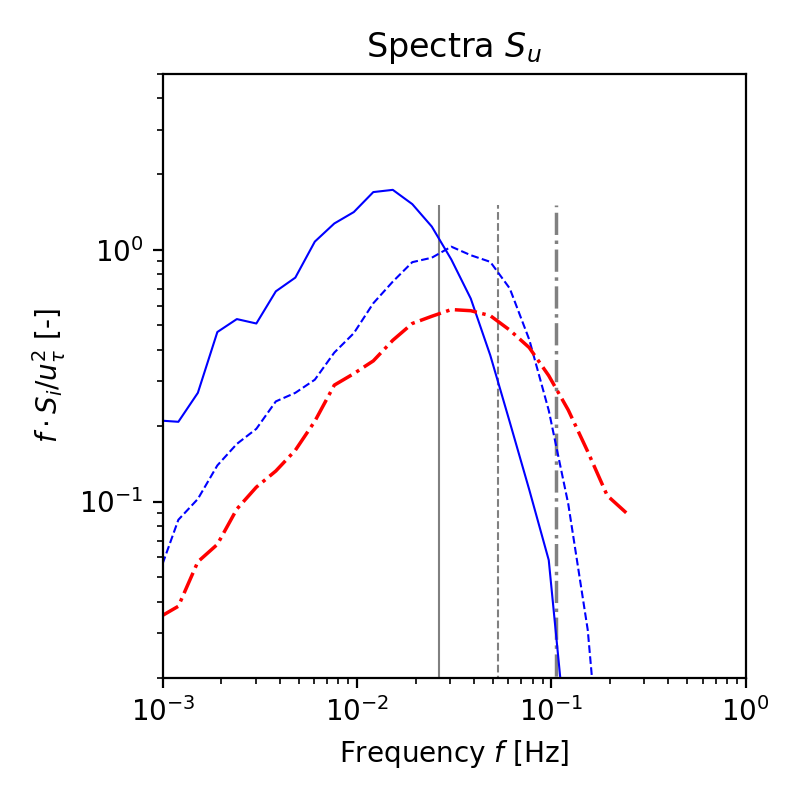
\includegraphics[width=2.0in]{figures/GridStudy_Spectra_Su.png}
  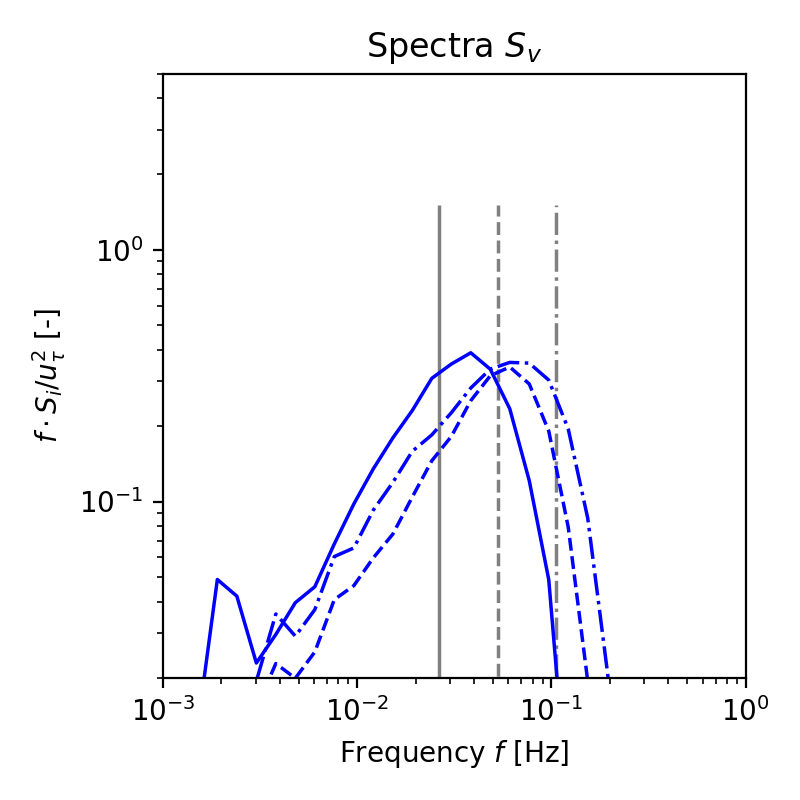
\includegraphics[width=2.0in]{figures/GridStudy_Spectra_Sv.png}
  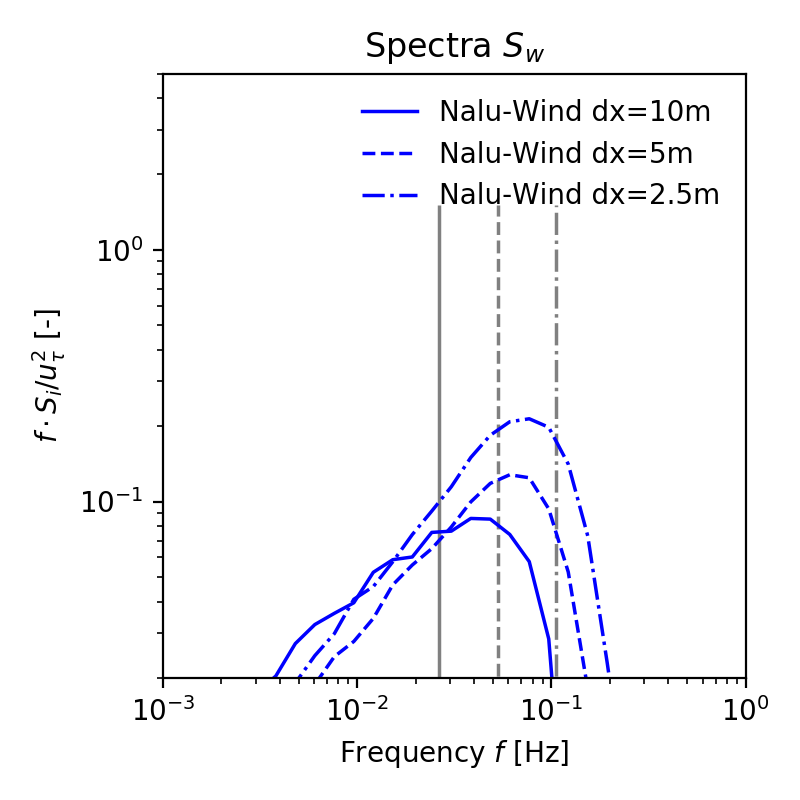
\includegraphics[width=2.0in]{figures/GridStudy_Spectra_Sw.png}
  \caption{   \label{fig:GridStudySpectra} 
    Calculation of the wind spectra $S_i$ for LES of stable
    5m/s case with different resolutions.  The gray vertical lines
    correspond to the maximum resolvable frequency $f_{max}$ according
    to equation (\ref{eq:fmax}). }
\end{figure}
%%%%%%%%%%%%%%%%%%%%%%%%%%%%%%%%%%%%%%%%%%%%%%%%%%%%%%%%%%%%%%%%%%%%

Two numerical constraints limit the maximum resolvable frequency in
the current ABL computations.  First, the Nyquist frequency $f_{Ny}$
limits the highest resolved frequency to half the sampling frequency, or

\begin{equation}
  f_{Ny} = \frac{1}{2\times \textrm{dt}}
\end{equation}
Secondly, the maximum resolvable frequency of convecting fine scale
eddies on a mesh with grid size $\Delta$ and average horizontal wind
speed $\bar{U}_{horiz}$ can be estimated as
\begin{equation}
  \label{eq:fmax}
  f_{max} = \frac{0.6\bar{U}_{horiz}}{N\Delta}.
\end{equation}
Here, equation \ref{eq:fmax} assumes that the turbulent eddies convect
with a velocity of $0.6\bar{U}_{horiz}$ and $N=8$ is chosen for the
purposes of this study.  Due to the alignment of the flow with the
mesh directions, the grid size $\Delta = \sqrt{2}\cdot \textrm{dx}$.
In all cases considered here, $f_{max} < f_{Ny}$, so the limiting
constraint for resolving the high frequency components was the mesh
resolution.

The comparison of the wind spectra and maximum resolvable frequency
$f_{max}$ for the different mesh resolutions is shown in figure
\ref{fig:GridStudySpectra}.  Here spectra is shown at the $z$=20m
height and averaged using 1/3 octave-bins to enchance clarity. For the
$S_u$ and $S_w$ spectra, there noticeable shifts in the peak
amplitude, while the peak amplitudes for $S_v$ remained fairly
constant between cases.  In all cases, the peak frequency of $S_i(f)$
also increased as the resolution increased. While the mesh resolution
was sufficient to capture the peak frequency for $S_u$, the fine
resolution with 2.5m mesh cells was required to capture the spectral
peaks in the lateral and vertical directions.

The second metric for determining the appropriate grid size and mesh
resolution is through the correlation tensor and turbulence integral
length scale.  The two-point correlation tensor
$R_{ij}(\mathbf{x},\boldsymbol{\xi})$ at position $\mathbf{x}$ and
separation vector $\boldsymbol{\xi}$ is defined as
\begin{equation}
  \label{eq:Rij}
  R_{ij}({\mathbf x},\boldsymbol{\xi}) = 
  \frac{\overline{ {u'_i(\mathbf{x}, t) u'_j(\mathbf{x}+\boldsymbol{\xi},t)} }}
       { \sqrt{\overline{ u'^2_i }} \sqrt{\overline{ u'^2_j}} }
\end{equation}
where the velocity fluctuations $u'_i$ are defined as 
\begin{equation}
  u'_i(\mathbf{x},t) = u_i(\mathbf{x},t) - \overline{ u_i(\mathbf{x},t) }
\end{equation}
and the overbar operator $\overline{(\bullet)}$ denotes time
averaging.  In the current study, we compute the horizontally averaged
correlation coefficient $\langle R_{11}(\boldsymbol{\xi})\rangle$ by
sampling over multiple points at the $z$=20m height, typically 100-150
points, and averaging the result.  The longitudinal $\langle
R_{11}(\boldsymbol{\xi})\rangle$ was calculated by looking at
separation vectors $\boldsymbol{\xi}$ in the streamwise direction
while the lateral $\langle R_{11}(\boldsymbol{\xi})\rangle$ used
separation distances $\boldsymbol{\xi}$ which were orthogonal to the
wind direction on the same horizontal plane.

%%%%%%%%%%% Grid resolution Rij correlation figure %%%%%%%%%%%%%%%%%%%%
% Created in Postprocessing/GridStudy/GridStudy_Rij.ipynb
\begin{figure}%[hbt!]
  \centering
  \fxnote{remove AMR-Wind results from graphs}\\
  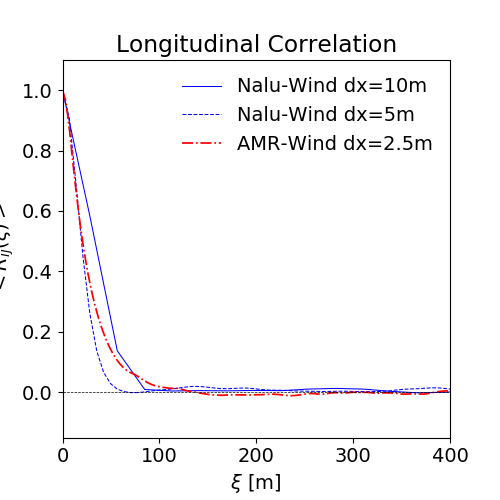
\includegraphics[width=2.5in]{figures/GridStudy_Rij_Longitudinal.png}
  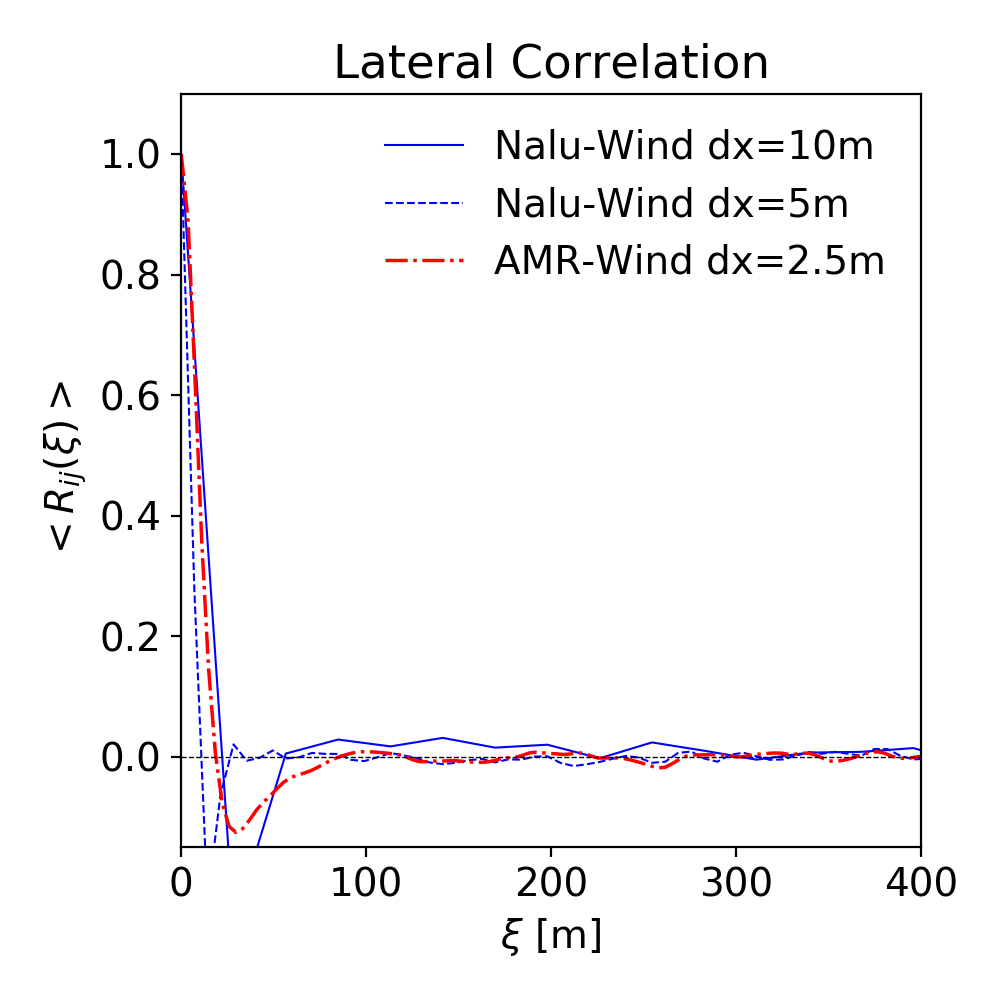
\includegraphics[width=2.5in]{figures/GridStudy_Rij_Lateral.png}
  \caption{\label{fig:GridStudyRij} Calculation of the averaged
    longitudinal and lateral $\langle R_{11}(\boldsymbol{\xi})
    \rangle$ coefficient at $z$=20m for LES of stable 5m/s case with
    different resolutions.}
\end{figure}
%%%%%%%%%%%%%%%%%%%%%%%%%%%%%%%%%%%%%%%%%%%%%%%%%%%%%%%%%%%%%%%%%%%%

The results shown in figure \ref{fig:GridStudyRij} show that the
finest resolution is required to resolve both the longitudinal and the
lateral length scale.  In contrast to the neutral and unstable ABL
cases, the turbulent structures decorrelate rapidly and are noticeably
finer in the lateral direction compared to the longitudinal direction.
While 2.5m resolution is adequate to resolve the longitudinal
turbulent structures, the lateral direction may require even finer
resolution to fully resolve.  This may be an important consideration
in situations where turbulence in a stable boundary layer interacts
with turbine features, such as blade motions or downstream wakes.
However, the additional refinement requires careful balancing against
the additional computational expense in the simulation.

Similar conclusions can be drawn by examining the turbulent integral
length scale $L$.  This lengthscale can be calculated from $\langle
R_{11}(\boldsymbol{\xi}) \rangle$ via
\begin{equation}
  L = \int_0^\infty \langle R_{11}(\xi) \rangle \: {\textrm d}\xi
\end{equation}
and the results are shown in table \ref{tab:GridStudyLscale}.  With a
resolution of 2.5m, the ratio of the longitudinal length scale to the
grid size $L/\textrm{d}x \approx 10.1$, while in the lateral direction
$L/\textrm{d}x \approx 2.36$, suggesting even finer resolution is
required to capture the lateral scales.

Based on this longitudinal length scale, we also determined the
overall domain size necessary for stable ABL calculations.  To provide
sufficient space to ensure development and decorrelation of turbulent
structures, domain sizes of approximately 10 times the longitudinal
lengthscale is recommended.  However, the inclusion of sample probes
with sufficient separation distance to accurately calculate $\langle
R_{11}(\boldsymbol{\xi}) \rangle$ roughly doubles the domain size
requirements.  Assuming the longitudinal length scales on the order of
30 m, we estimated a minimum domain size of 750m $\times$ 750m in the
horizontal directions for both the Nalu-Wind and AMR-Wind LES
calculations.

%%%%%%%%%%%%%%% GRID STUDY: INTEGRAL LENGTH %%%%%%%%%%%%%%%%%%%%%%%%%%%%%%%%%%%
\begin{table} %[h!]
\caption{\label{tab:GridStudyLscale} The calculated turbulent integral
  lengthscale for each of the grid resolutions} \centering
\begin{tabular}{ccccc}
  \hline
  Case              & dx [m] & Longitudinal L  & Lateral L \\
  \hline
  Nalu-wind coarse  &  10.0  & 36.4 m         & 0.0 m     \\
  Nalu-wind medium  &   5.0  & 21.5 m         & 4.52 m    \\
  Nalu-wind fine    &   2.5  & 25.3 m         & 5.92 m    \\
\hline
\end{tabular}
\end{table}

\subsection{Comparison of AMR-Wind vs Nalu-Wind}

%%%%%%%%%%%%%%% Compare Nalu/AMR integrated quantities %%%%%%%%%%%%%%
\begin{table}
\caption{\label{tab:CompareAMRvsNalu} Comparison of AMR-Wind and
  Nalu-Wind} \centering
\begin{tabular}{cccccc}
  \hline
  Code & Wind speed & TI      &  $\alpha$  &   $u_\tau$ \\ %&       L \\
  \hline
  Nalu-Wind & 5 m/s &  0.0481 &  0.165     &  0.163 m/s \\ %& 94.970836 \\
  AMR-Wind  & 5 m/s &  0.0483 &  0.166     &  0.157 m/s \\ %& 52.512434 \\
  \hline
\end{tabular}
\end{table}
%%%%%%%%%%%%%%%%%%%%%%%%%%%%%%%%%%%%%%%%%%%%%%%%%%%%%%%%%%%%%%%%%%%%

Before examining the behavior the offshore ABL across all wind speeds,
we first compare the results for a single case using both LES codes.
In this section, we consider the stable 5m/s case, calculated in the
same manner using both AMR-Wind and Nalu-Wind.  Both LES codes used a
mesh resolution of 2.5m based on the guidance from section
\ref{sec:gridstudy} and the computational resources available.

After running each case for 15,000 seconds, the boundary layer
statistics and horizontally averaged profiles were averaged for
another 5,000 seconds.  In table \ref{tab:CompareAMRvsNalu}, some mean
statistics are given for both cases, including the friction velocity
$u_\tau$, the turbulence intensity TI at z=20m, and local shear
exponent $\alpha$ at z=20m, defined as
$$ \alpha = \frac{z}{U_{horiz}} \frac{d U_{horiz}}{dz}.
$$ AMR-Wind and Nalu-Wind produced nearly identical values for the
TI=0.048, which is close to measured target of 4.5\%, and similar
agreement was found for the shear exponent $\alpha$.  A minor
descrepancy was found in the friction velocity $u_\tau$, with AMR-Wind
resulting in a value slightly lower than Nalu-Wind.

The comparison of the horizontally averaged wind profiles is shown in
figure \ref{fig:CompareAMRvsNaluWind_WSDir}.  At the forcing height
z=20m, the wind speed and wind shear match are close to an exact match
between the two LES codes.  The horizontal wind speeds continue to
agree well for $z$<100m, beyond which a relatively constant velocity
difference is observed.   For both AMR-Wind and Nalu-Wind, an
approximately linear veer profile was observed until $z\approx$ 250m,
at which point the wind direction remained constant until the
inversion layer height.

The computed TI and temperature profiles were observed to agree
remarkably well between the LES codes. As shown in figure
\ref{fig:CompareAMRvsNaluWind_TTI}, the stable ABL computed using
AMR-Wind and Nalu-Wind both show a similar decay of turbulent kinetic
energy with altitude $z$, and there is also little difference between
the two temperature profiles $T(z)$.

%%%%%%%%%%% Compare Nalu/AMR WS/WDir profiles %%%%%%%%%%%%%%%%%%%%%%%
% Postprocessing/ABLStats/AMRWind_NaluWind_stable_05ms_mesh2_5x2_5x2_5_paper.ipynb
\begin{figure} %[hbt!]
  \centering
  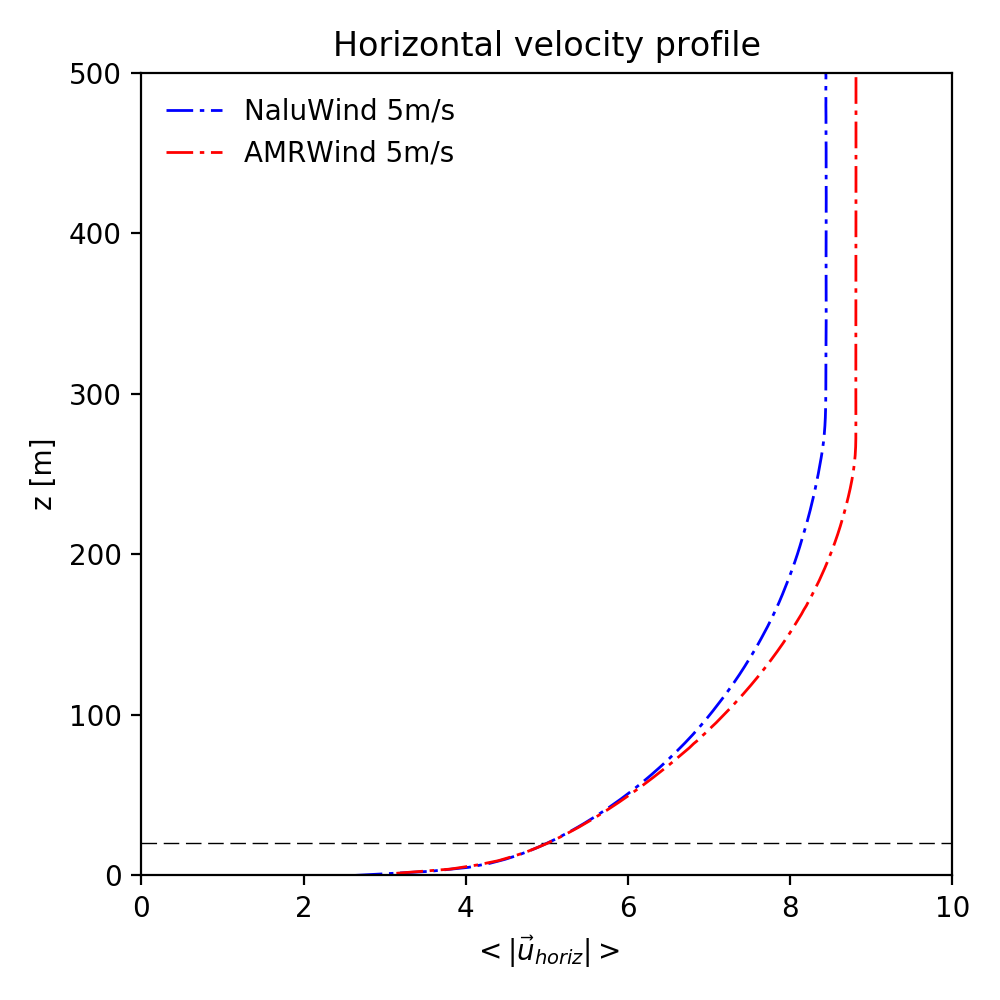
\includegraphics[width=2.5in]{figures/Compare_AMRWind_NaluWind/AMRWind_NaluWind_stable_05ms_mesh2p5_2p5_2p5_WS.png}
  \includegraphics[width=2.5in]{figures/Compare_AMRWind_NaluWind/AMRWind_NaluWind_stable_05ms_mesh2p5_2p5_2p5_Wdir.png}\\
  \caption{\label{fig:CompareAMRvsNaluWind_WSDir} Comparison of
    AMR-Wind and Nalu-Wind velocity profiles for the stable 5 m/s
    boundary layer. The dashed horizontal line corresponds to the
    measurement height z=20m. }
\end{figure}
%%%%%%%%%%%%%%%%%%%%%%%%%%%%%%%%%%%%%%%%%%%%%%%%%%%%%%%%%%%%%%%%%%%%

%%%%%%%%%%% Compare Nalu/AMR TI/Temp profiles %%%%%%%%%%%%%%%%%%%%%%
% Postprocessing/ABLStats/AMRWind_NaluWind_stable_05ms_mesh2_5x2_5x2_5_paper.ipynb
\begin{figure} [hbt!]
  \centering
  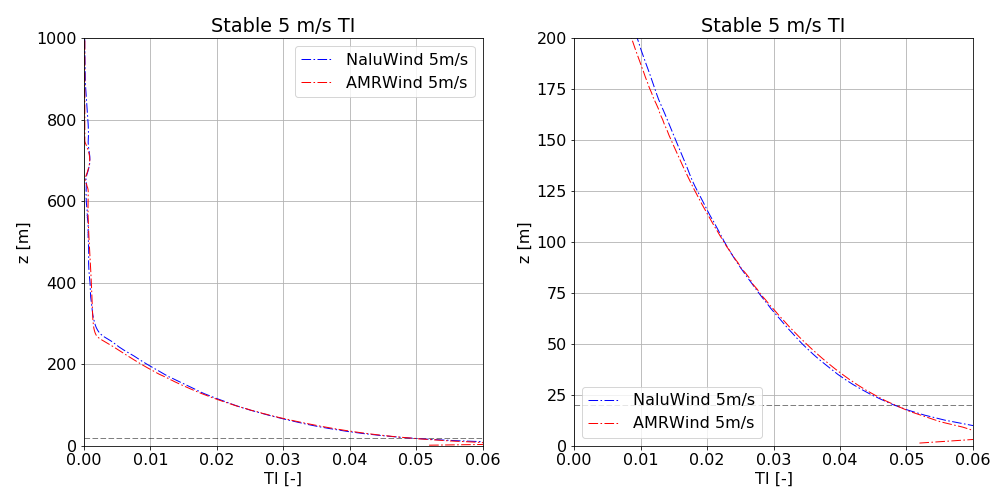
\includegraphics[width=2.5in]{figures/Compare_AMRWind_NaluWind/AMRWind_NaluWind_stable_05ms_mesh2p5_2p5_2p5_TI.png}
  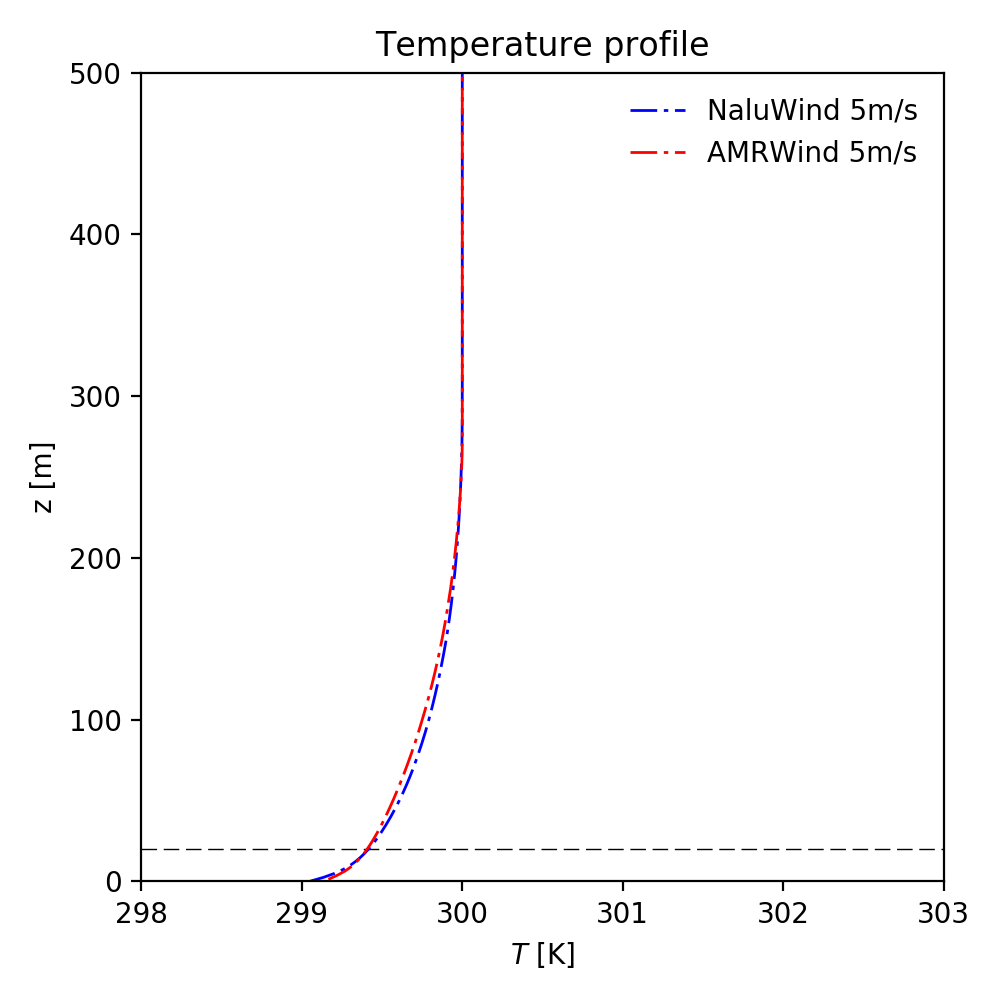
\includegraphics[width=2.5in]{figures/Compare_AMRWind_NaluWind/AMRWind_NaluWind_stable_05ms_mesh2p5_2p5_2p5_T.png}
  \caption{\label{fig:CompareAMRvsNaluWind_TTI} Comparison of AMR-Wind
    and Nalu-Wind turbulence intensity and temperature profiles for
    the stable 5 m/s boundary layer. The dashed horizontal line
    corresponds to the measurement height z=20m.}
\end{figure}
%%%%%%%%%%%%%%%%%%%%%%%%%%%%%%%%%%%%%%%%%%%%%%%%%%%%%%%%%%%%%%%%%%%%

In addition to the mean profiles described above, we also examined the
wind spectra and turbulent correlation statistics from both AMR-Wind
and Nalu-Wind for the stable 5m/s case.  A comparison of the computed
wind spectra $S_i(f)$ from both LES codes is shown in figure
\ref{fig:CompareAMRvsNaluSpectra}.  At low frequencies, both AMR-Wind
and Nalu-Wind predict similar spectral behavior, and both codes
predict relatively similar spectral peaks for the $S_v$ and $S_w$
spectra.  For the longitudinal spectra $S_u$, however, AMR-wind
predicts a slightly lower the peak amplitude than Nalu-Wind.

%%%%%%%%%%% Compare Nalu/AMR spectra %%%%%%%%%%%%%%%%%%%%%%%%%%%%%%%%
% Postprocessing/ABLSpectra/AMRWind_NaluWind_Spectra_Stable.ipynb
\begin{figure} %[hbt!]
  \centering
  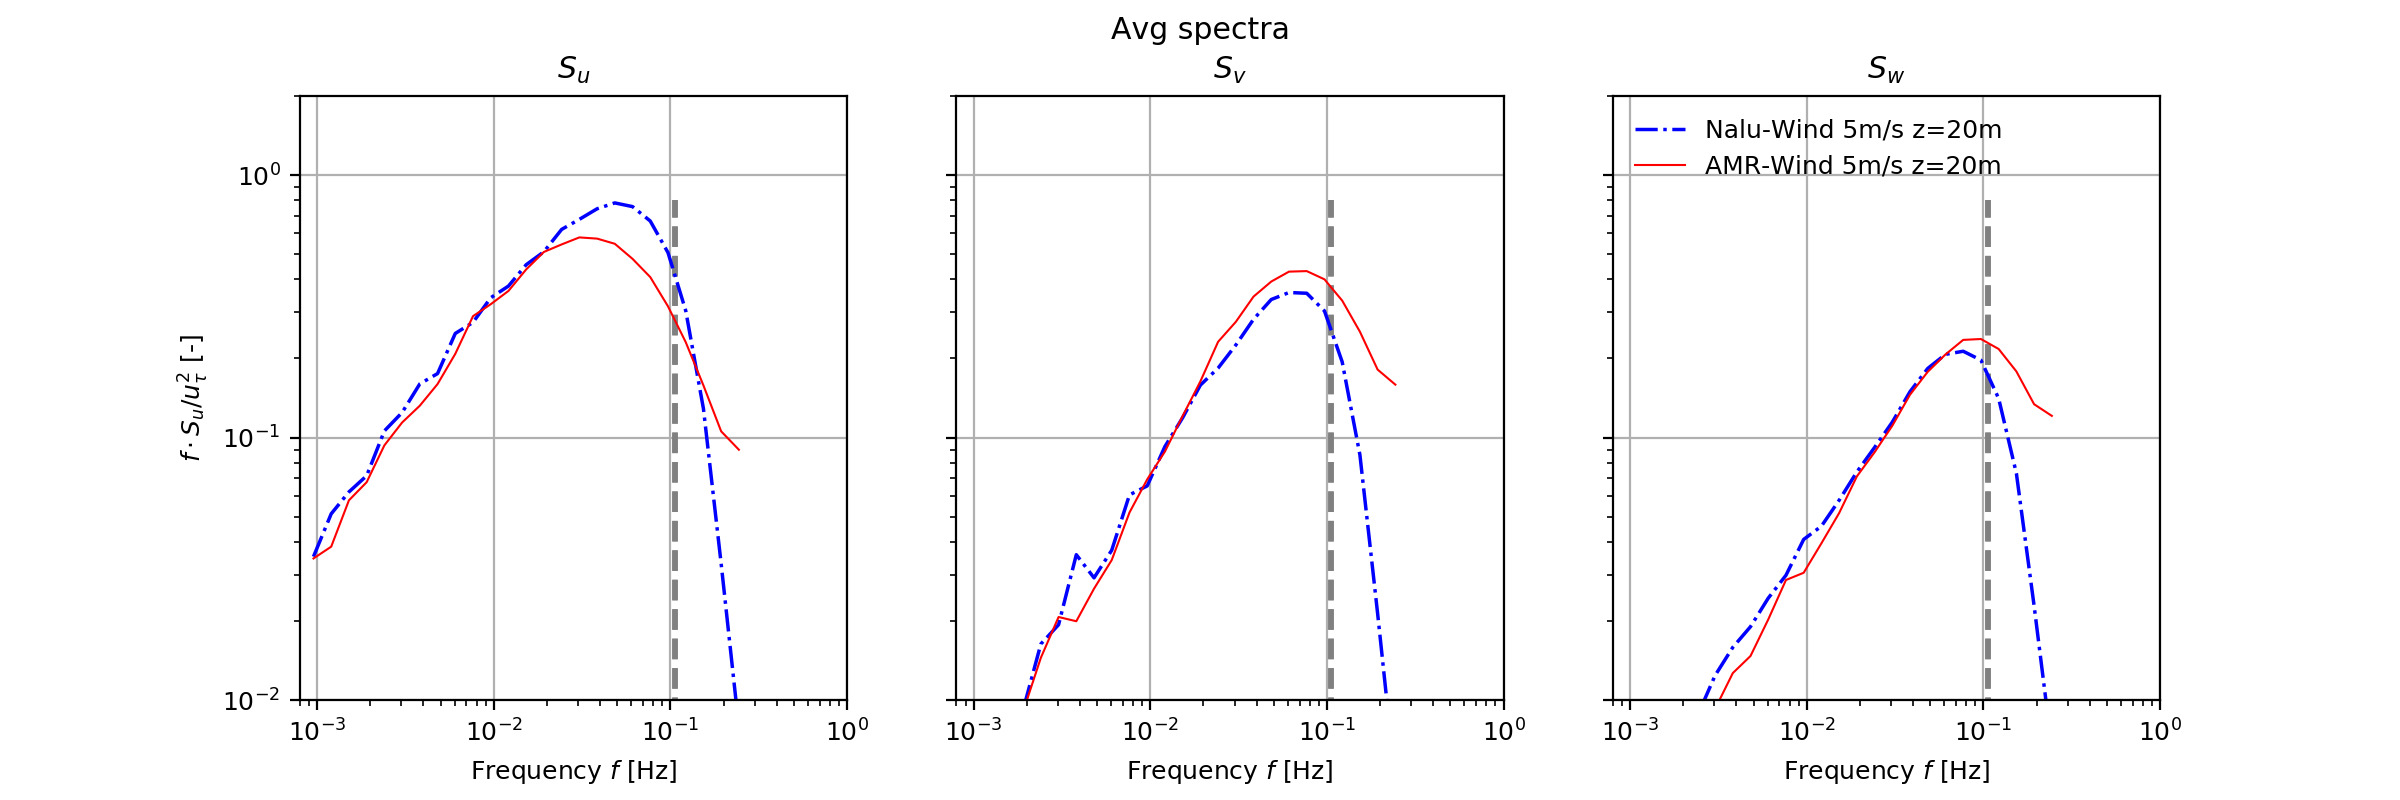
\includegraphics[width=7.0in]{figures/Compare_AMRWind_NaluWind/AMRWind_NaluWind_Spectra_Stable_z20.png}

  \caption{\label{fig:CompareAMRvsNaluSpectra} Comparison of AMR-Wind
    and Nalu-Wind wind spectra at z=20m for the stable 5 m/s boundary
    layer. }
\end{figure}
%%%%%%%%%%%%%%%%%%%%%%%%%%%%%%%%%%%%%%%%%%%%%%%%%%%%%%%%%%%%%%%%%%%%

%% A comparison of the averaged $\langle R_{11}(\boldsymbol{\xi})\rangle$
%% correlation coefficient is shown in figure \ref{fig:CompareAMRvsNaluRij}.

%% %%%%%%%%%%% Compare Nalu/AMR lengthscale %%%%%%%%%%%%%%%%%%%%%%%%%%%%
%% % Postprocessing/ABLLength/CompareAMRNalu_ABL_Lengthscales.ipynb
%% \begin{figure} %[hbt!]
%%   \centering
%%   \fxnote{UPDATE THIS FIGURE}\\
%%   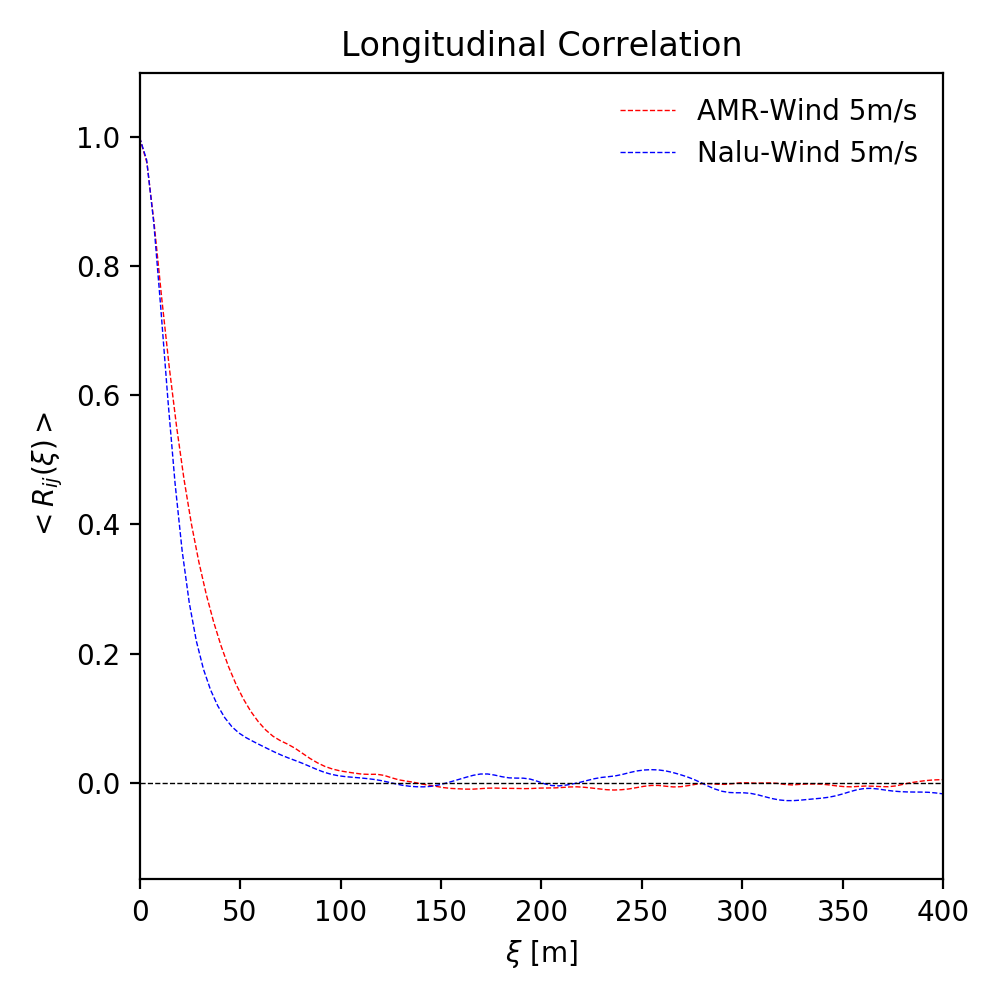
\includegraphics[width=2.5in]{figures/Compare_AMRWind_NaluWind/AMRWind_NaluWind_Lengthscale_Stable_z20_Longitudinal.png}
%%   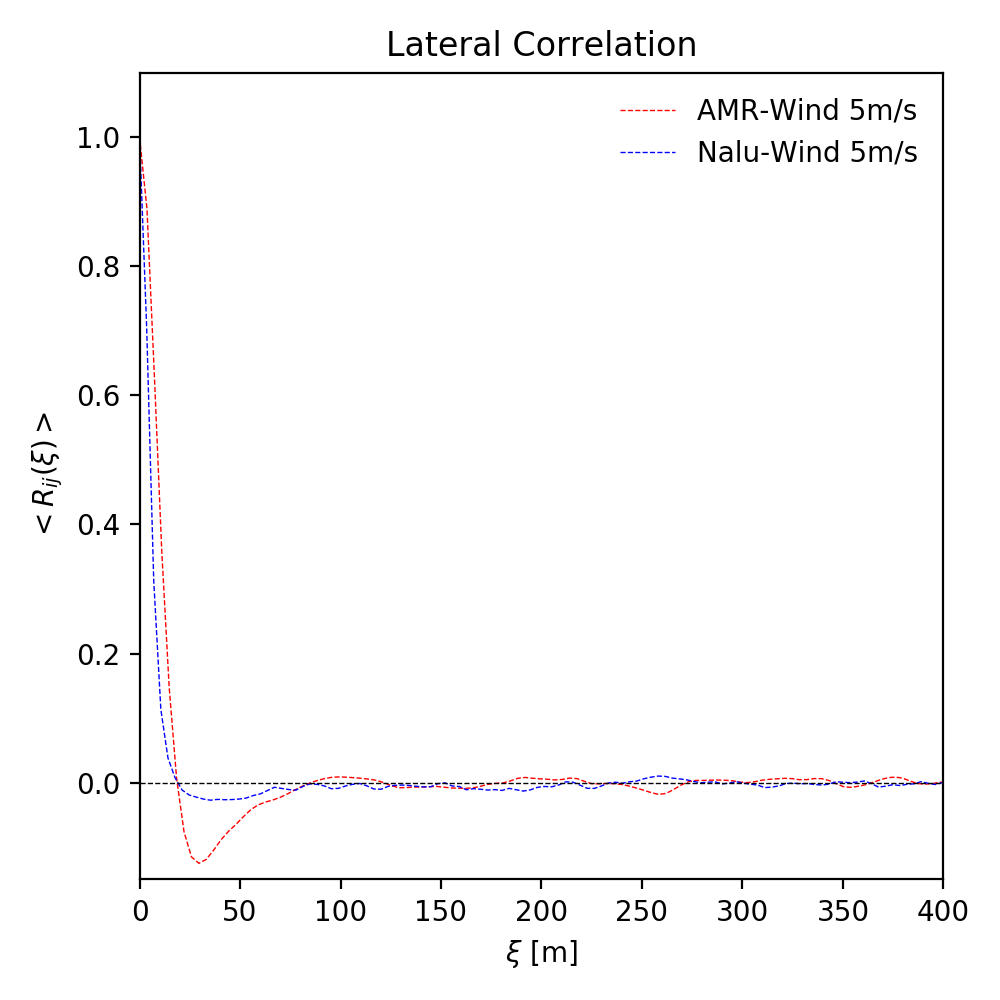
\includegraphics[width=2.5in]{figures/Compare_AMRWind_NaluWind/AMRWind_NaluWind_Lengthscale_Stable_z20_Lateral.png}

%%   \caption{\label{fig:CompareAMRvsNaluRij}
%%     Comparison of AMR-Wind and Nalu-Wind $\langle R_{11}
%%     \rangle$ correlation at z=20m. }
%% \end{figure}
%% %%%%%%%%%%%%%%%%%%%%%%%%%%%%%%%%%%%%%%%%%%%%%%%%%%%%%%%%%%%%%%%%%%%%

\subsubsection{Computational efficiency}
How much faster is AMR-Wind compared to Nalu-Wind?  \\
\fxnote{PUT SOME NUMBERS HERE FROM MIKE}

\subsection{Comparison of stable offshore ABL for different wind speeds and stabilities}

Using the results of the stable cases described in \ref{sec:CFDsetup},
as well as the computations from the previous study in
\cite{cheung2020large}, we can examine the influence of wind speed and
stratification on offshore ABL behavior.  In this section we first
compare the differences between the three stable ABL cases, and then
compare their behavior with the previously computed neutral and
unstable counterparts.

\subsubsection{\label{sec:stableABLStats} ABL integrated quantities}
From the AMR-Wind calculations of the stable ABL at 5m/s, 10m/s, and
15m/s, a number of quantities can be computed to compare with the
measured targets from Archer et al \cite{archer2016predominance}.  In
table \ref{tab:CompareAMRallWS}, we list the TI, shear exponent
$\alpha$, friction velocity $u_\tau$, Obukhov length $L_{Ob}$,
longitudinal lengthscale $L$, and stability classification for each of
these three cases.  The TI values, calculated at the height $z$=20m
fall within the target range of 4.5\% to 6.0\% for stable conditions
from the Cape Wind measurements.  The calculated friction velocities
are also similar to the values from the neutral offshore ABL
calculations of \cite{cheung2020large}, where $u_\tau$ varied from
0.15 m/s to 0.51 m/s for wind speeds of 5 m/s to 15 m/s.

The degree of stratification in each of the marine boundary layers can
be quantified through the Obukhov length $L_{Ob}$, defined here as 
\begin{equation}
  L_{Ob} = -\frac{u_\tau^3 T_0}{\kappa g \langle \overline{w'T'} \rangle}
\end{equation}
where the $\kappa$=0.41 is the Kolmogorov constant, $g$ is the
gravitational acceleration, $T_0$ is the reference temperature, and
$\langle \overline{w'T'} \rangle$ is the horizontally and
time-averaged temperature flux.  In this study we adopt the same
classification guidelines as Archer et al
\cite{archer2016predominance}, and identify boundary layer cases where
$100 < L_{Ob} < 500$ as ``stable'', and cases where $5 < L_{Ob}<100$
as ``very stable''.  From the values listed in table
\ref{tab:CompareAMRallWS}, we find that the lower wind speeds are
``very stable'', while the highest 15 m/s wind speed is classified as
``stable''.  This is consistent with the measured Cape Wind
distributions, where very stable conditions are more frequent than
stable conditions at lower wind speeds, and gradually disappear beyond
13 m/s (c.f. figure 5b in \cite{archer2016predominance}).

%%%%%%%%%%%%%%% Compare AMR integrated quantities, all WS %%%%%%%%%%%%%%
% See Postprocessing/ABLStats/AMRWind_NaluWind_stable_AllWS_2p5Cubed.ipynb
\begin{table}
\caption{\label{tab:CompareAMRallWS} Comparison of Stable ABL for all
  wind speeds} \centering
\begin{tabular}{cccccccc}
  \hline
  Code & Wind speed   & TI     & $\alpha$& $u_\tau$ & Obukhov $L_{Ob}$ & Longitudinal $L$ & Stability \\
  \hline
  AMRWind & 5m/s      & 0.0483 &  0.166 &  0.157 m/s  &  52.5 m & 27.7 m  & Very stable\\
  AMRWind & 10m/s     & 0.0506 &  0.160 &  0.319 m/s  &  57.2 m & 29.6 m  & Very stable\\
  AMRWind & 15m/s     & 0.0550 &  0.118 &  0.511 m/s  & 131.3 m & 43.8 m  & Stable \\
  \hline
\end{tabular}
\end{table}
%%%%%%%%%%%%%%%%%%%%%%%%%%%%%%%%%%%%%%%%%%%%%%%%%%%%%%%%%%%%%%%%%%%%

\subsubsection{Flow behavior and horizontally averaged profiles}

The qualitative behavior of the stable boundary layers can be seen
through snapshots of the flow taken from each of the simulations.  In
figure \ref{fig:SnapshotsZ20}, instantaneous snapshots of the
horizontal and vertical velocities for each of the three cases at the
z=20m measurement height are shown.  The largest difference can be
seen in the size of the flow structures between the very unstable and
stable cases.  Longer streaks are evident in the 15 m/s case compared
to the 5 m/s and 15 m/s cases, which is consistent with the nearly
50\% larger integral lengthscale $L$ given in table
\ref{tab:CompareAMRallWS}.  The differences in the vertical velocity
are also evident in \ref{fig:SnapshotsZ20}.  At higher wind speeds the
magnitude of the vertical $w'$ fluctuations increase, which plays a
strong role in the growth the boundary layer.

%%%%%%%%%%% z=20m snapshot pics %%%%%%%%%%%%%%%%%%%%%%%%%
% Created in Postprocessing/ABLStats/AMRWind_NaluWind_stable_AllWS_2p5Cubed.ipynb
\begin{figure}[hbt!]
  \centering
  \fxnote{label plots using pstricks: 5m/s on top, 15m/s on bottom} \\
  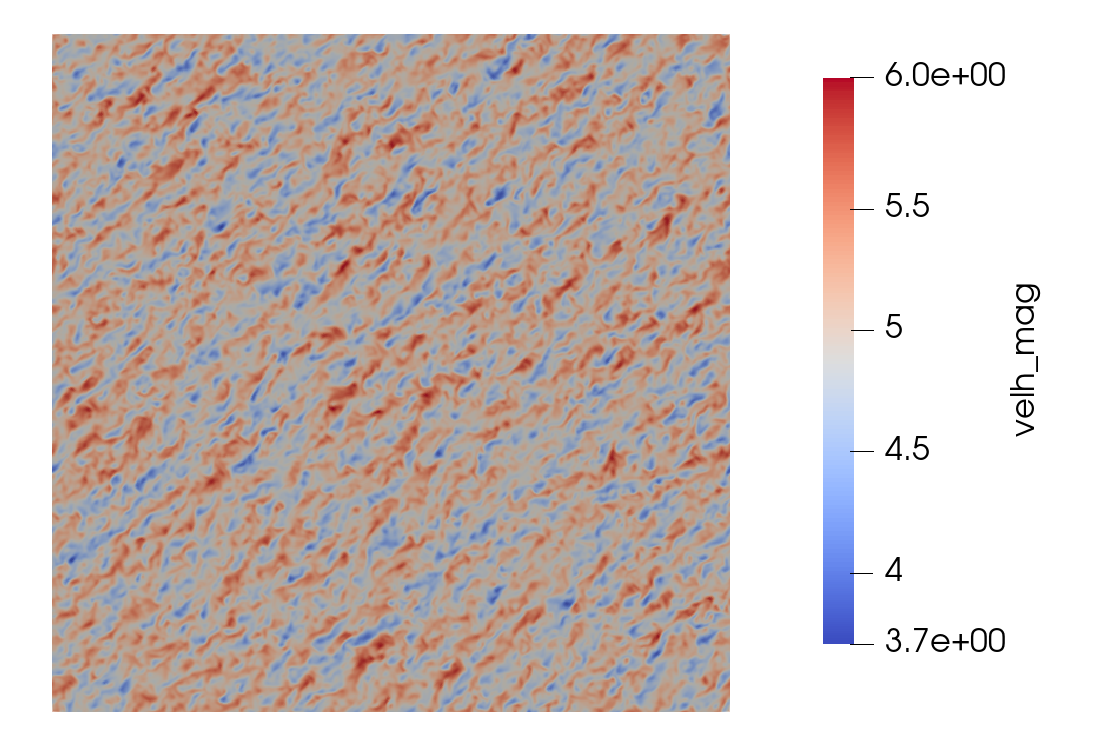
\includegraphics[width=3.0in]{figures/snapshots/05ms/velh_mag_z20.png}
  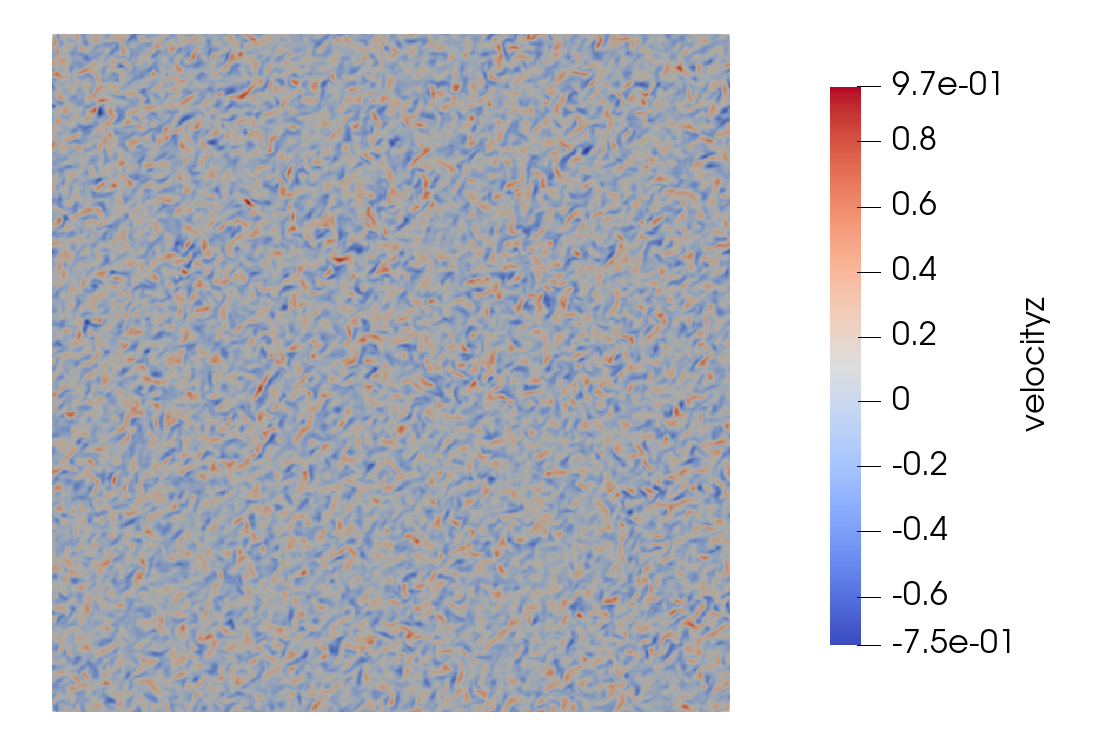
\includegraphics[width=3.0in]{figures/snapshots/05ms/velz_z20.png} \\
  
  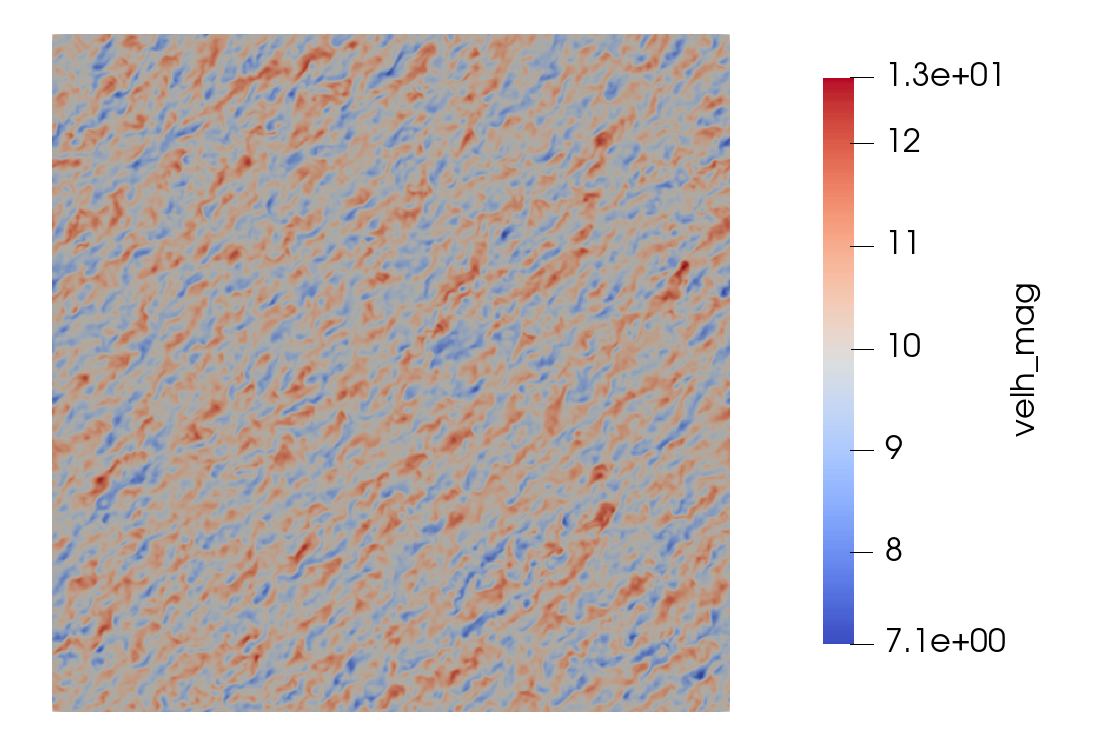
\includegraphics[width=3.0in]{figures/snapshots/10ms/velh_mag_z20.png}
  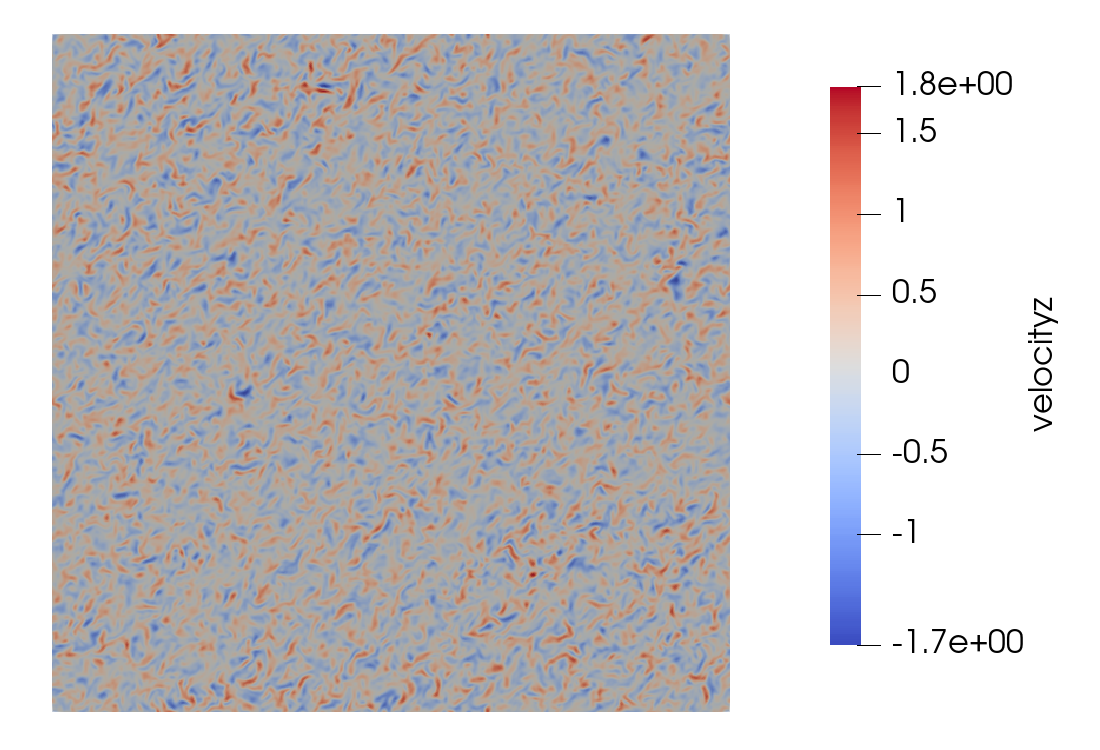
\includegraphics[width=3.0in]{figures/snapshots/10ms/velz_z20.png} \\
  
  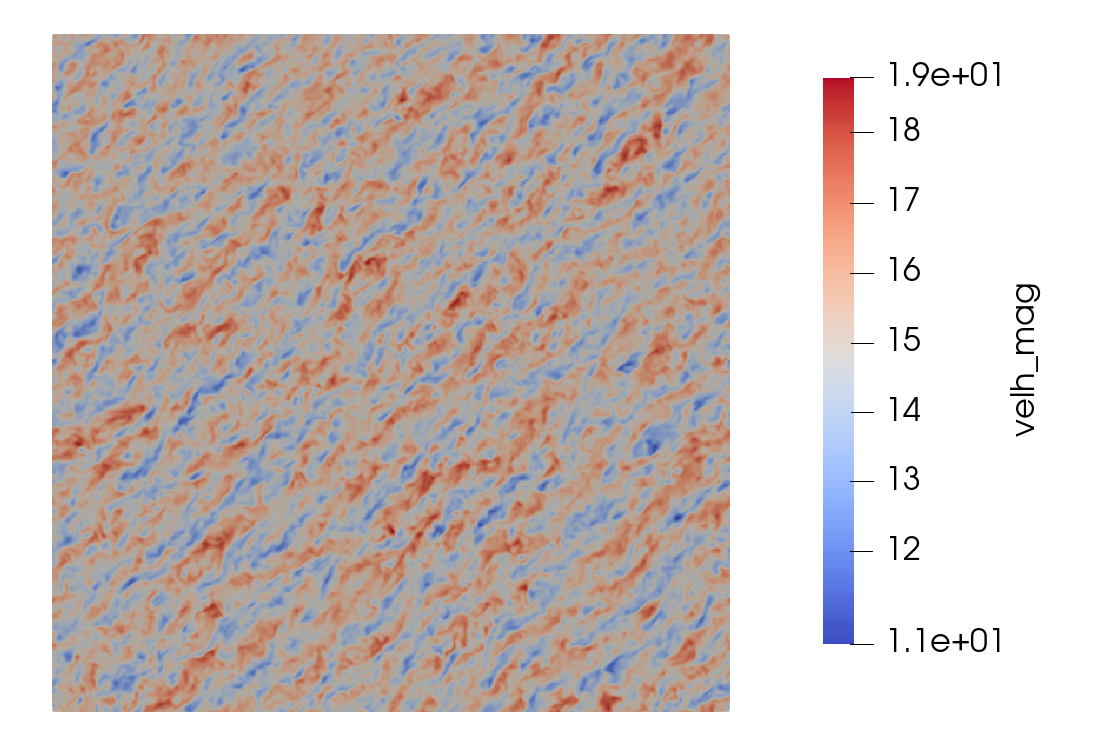
\includegraphics[width=3.0in]{figures/snapshots/15ms/velh_mag_z20.png}
  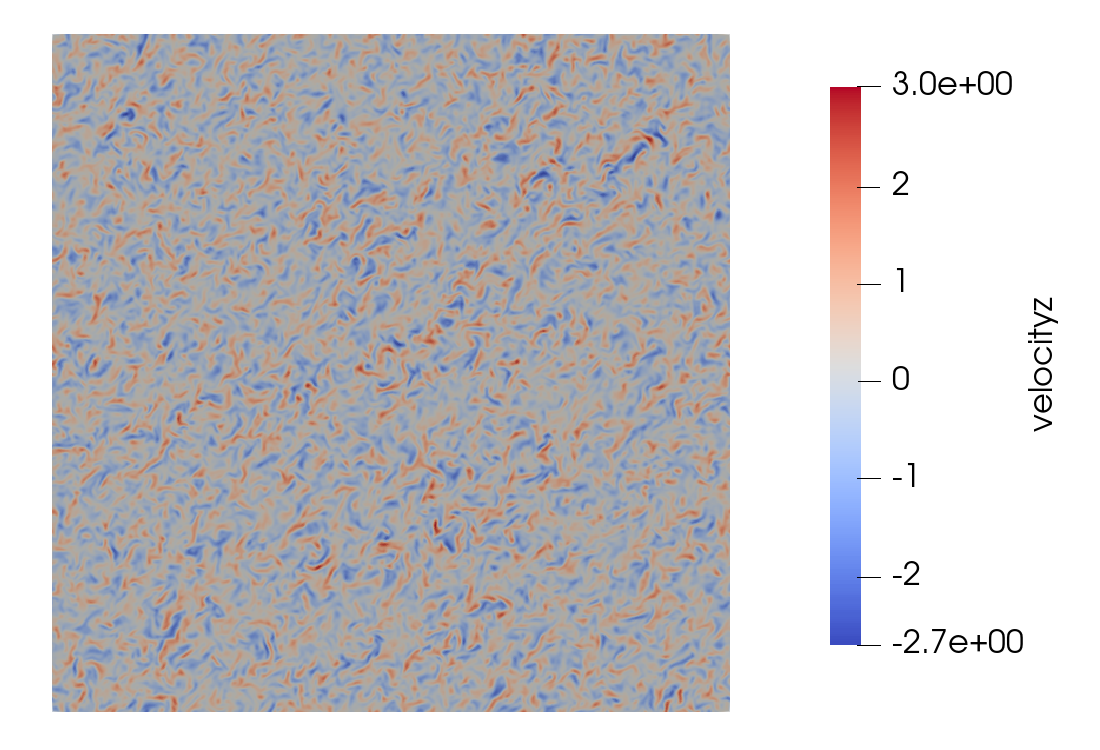
\includegraphics[width=3.0in]{figures/snapshots/15ms/velz_z20.png} \\
  \caption{ \label{fig:SnapshotsZ20} Snapshots of the horizontal
    velocity and vertical velocity, taken at t=20,000 seconds of the
    simulations at height z=20m.}
\end{figure}
%%%%%%%%%%%%%%%%%%%%%%%%%%%%%%%%%%%%%%%%%%%%%%%%%%%%%%%%%%%%%%%%%%%%

This observation can also be seen in images taken along the flow
direction $\theta=225^\circ$, as shown in figure
\ref{fig:SnapshotsSide}.  At the time t=20,000 seconds, the growth the
of 15 m/s stable boundary layer is considerably larger than the very
stable 5 m/s and 10 m/s cases, and has nearly reached the inversion
layer height.  To reach the same level of boundary layer growth, the
very stable ABL cases would require longer simulation times, possibly
longer than the nighttime conditions measured experimentally.

%%%%%%%%%%% side snapshot pics %%%%%%%%%%%%%%%%%%%%%%%%%
% Created in Postprocessing/ABLStats/AMRWind_NaluWind_stable_AllWS_2p5Cubed.ipynb
\begin{figure}[hbt!]
  \centering
  \fxnote{label plots using pstricks: 5m/s on top, 15m/s on bottom} \\
  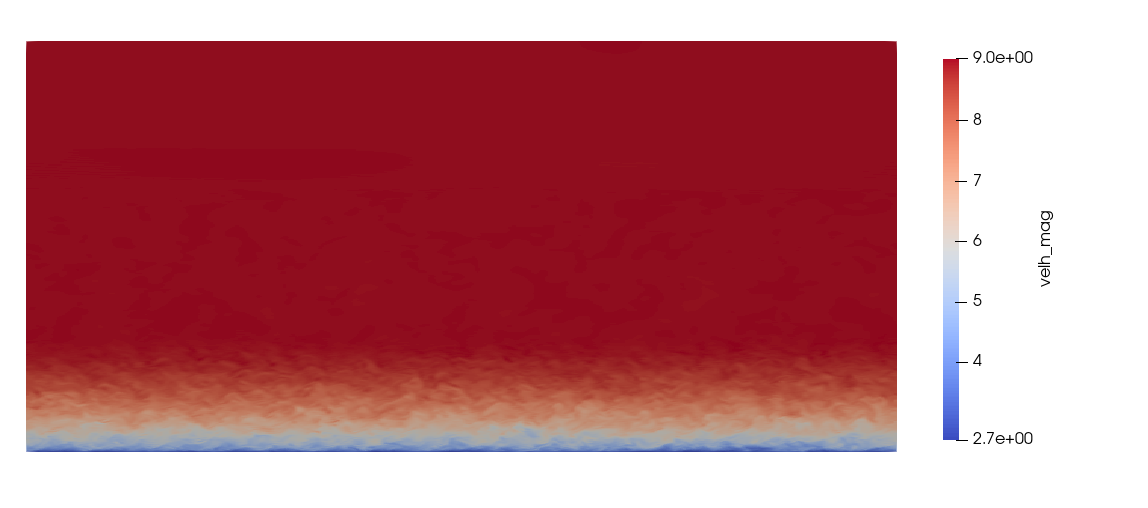
\includegraphics[height=2.5in]{figures/snapshots/05ms/velh_mag_side.png} \\

  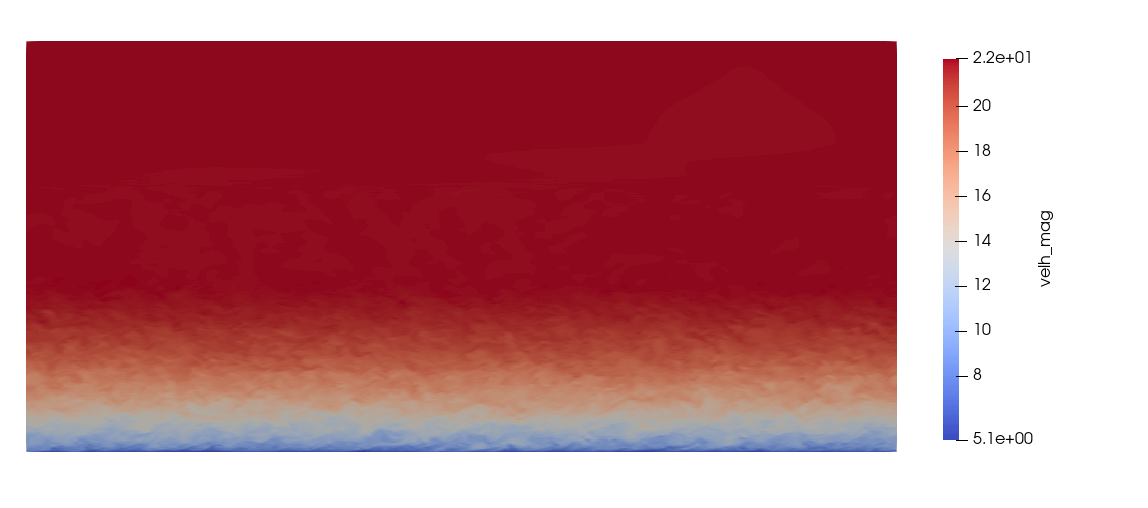
\includegraphics[height=2.5in]{figures/snapshots/10ms/velh_mag_side.png} \\

  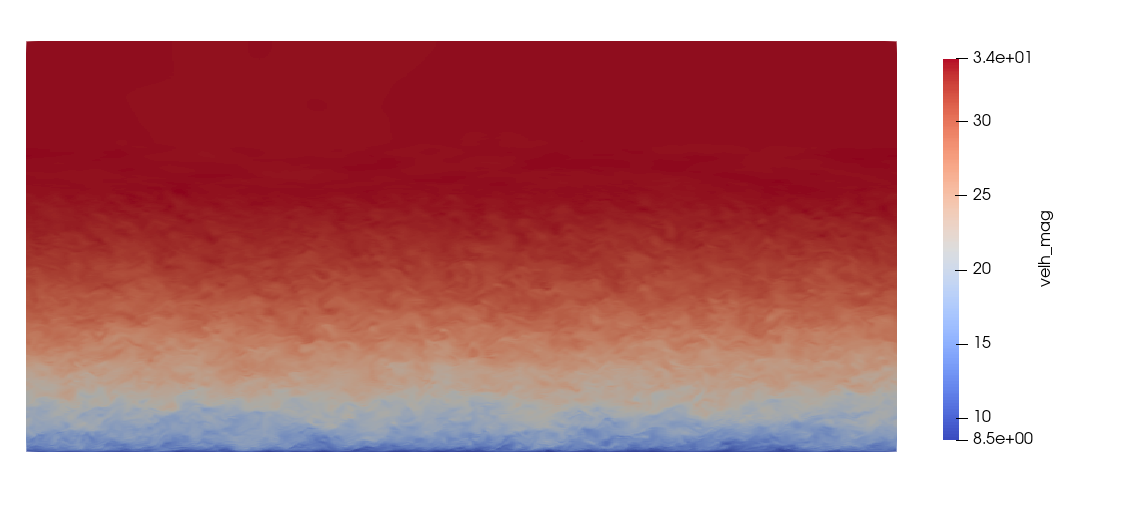
\includegraphics[height=2.5in]{figures/snapshots/15ms/velh_mag_side.png} \\
    
  \caption{ \label{fig:SnapshotsSide} Snapshots of the horizontal
    velocity, taken at t=20,000 seconds along the wind direction. }
\end{figure}
%%%%%%%%%%%%%%%%%%%%%%%%%%%%%%%%%%%%%%%%%%%%%%%%%%%%%%%%%%%%%%%%%%%%

Horizontally averaged flow profiles shown in figures
\ref{fig:CompareAMRallWS} and \ref{fig:CompareAMRallTTI} provide a
more quantitative assessment of the ABL evolution.  The rapid growth
of the 15 m/s stable case leads to strong shear throughout the
boundary layer up to the inversion height, while the very stable 5 m/s
and 10 m/s cases showed minimal shear at higher elevations.  The
change in wind direction is also indicative of the boundary layer
penetration.  Approximately linear veer profiles are visible up to
heights of $z\approx$250 m and $z\approx$350 m for the 5 m/s and 10
m/s cases, respectively, while the linear veer is present in the 15
m/s stable case up to $z$=650m.

The behavior of the TI and temperature profiles in figure
\ref{fig:CompareAMRallTTI} closely follows the shear and veer profiles
discussed above.  Despite all cases reaching a similar TI levels at
$z$=20m, the turbulence decays at different rates for each case until
reaching the top of the boundary layer.  The effect of the different
surface temperature changes is also visible in the horizontally
averaged temperature profiles.  Both the 10 m/s and 15 m/s impose
similar temperature changes (-1.4 K/hr and -1.5 K/hr, respectively)
and each similar temperatures at the ocean surface.  However, the
cooling effect in the very unstable 10 m/s case is limited to $z$<350
m, similar to the veer and turbulence profiles.

%%%%%%%%%%% stable WS profiles %%%%%%%%%%%%%%%%%%%%%%%%%
% Created in Postprocessing/ABLStats/AMRWind_NaluWind_stable_AllWS_2p5Cubed.ipynb
\begin{figure}[hbt!]
  \centering
  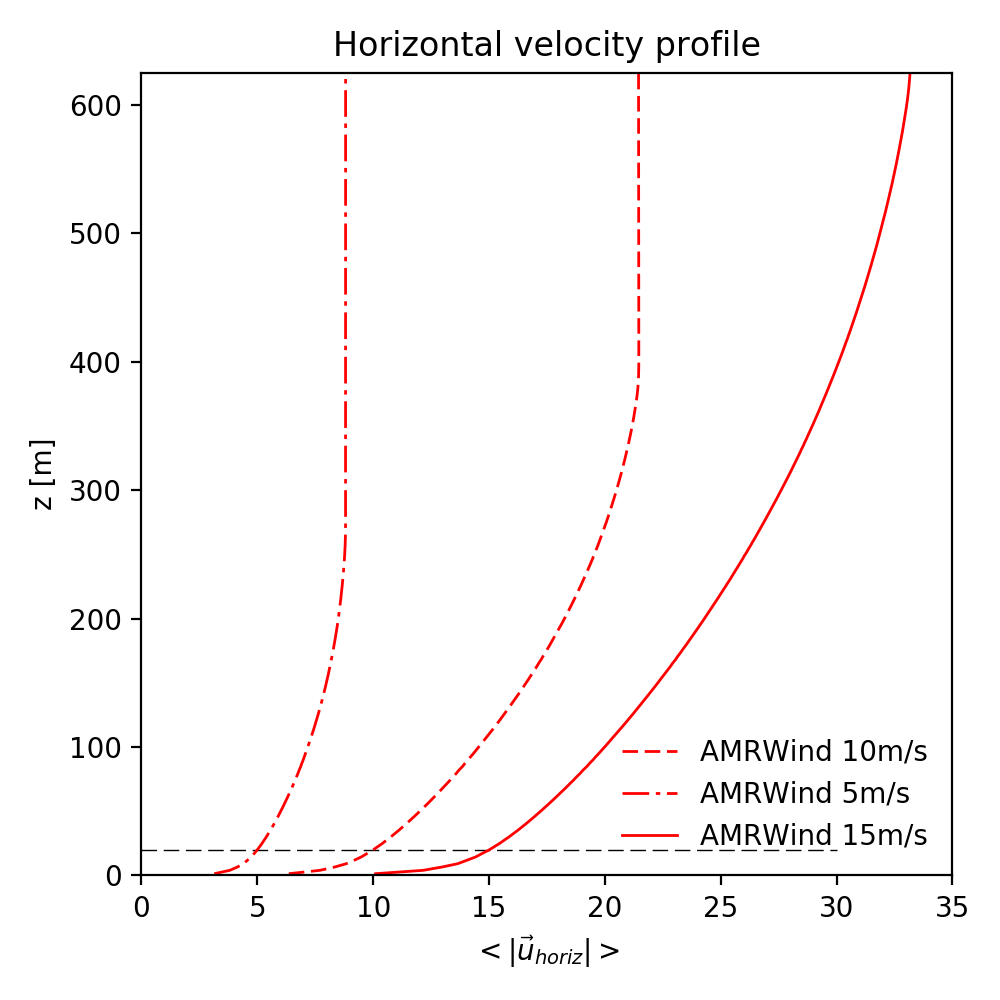
\includegraphics[width=2.5in]{figures/AMRWind_allWS/AMRWind_stable_WS.png}
  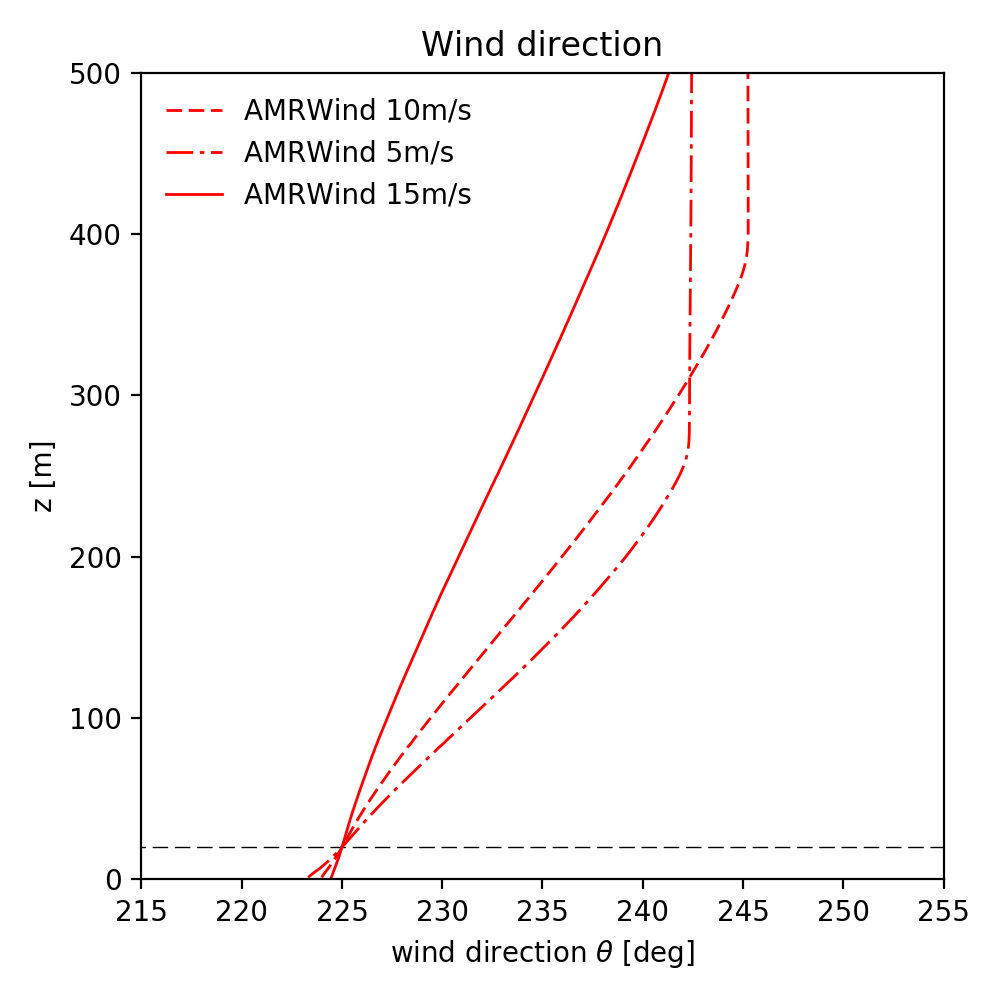
\includegraphics[width=2.5in]{figures/AMRWind_allWS/AMRWind_stable_WDir.png}
  \caption{ \label{fig:CompareAMRallWS} Comparison of the horizontal
    wind speed and wind direction profile for the stable 5m/s, 10m/s,
    and 15m/s boundary layers. }
\end{figure}
%%%%%%%%%%%%%%%%%%%%%%%%%%%%%%%%%%%%%%%%%%%%%%%%%%%%%%%%%%%%%%%%%%%%

%%%%%%%%%%% stable WS profiles %%%%%%%%%%%%%%%%%%%%%%%%%
% Created in Postprocessing/ABLStats/AMRWind_NaluWind_stable_AllWS_2p5Cubed.ipynb
\begin{figure}[hbt!]
  \centering
  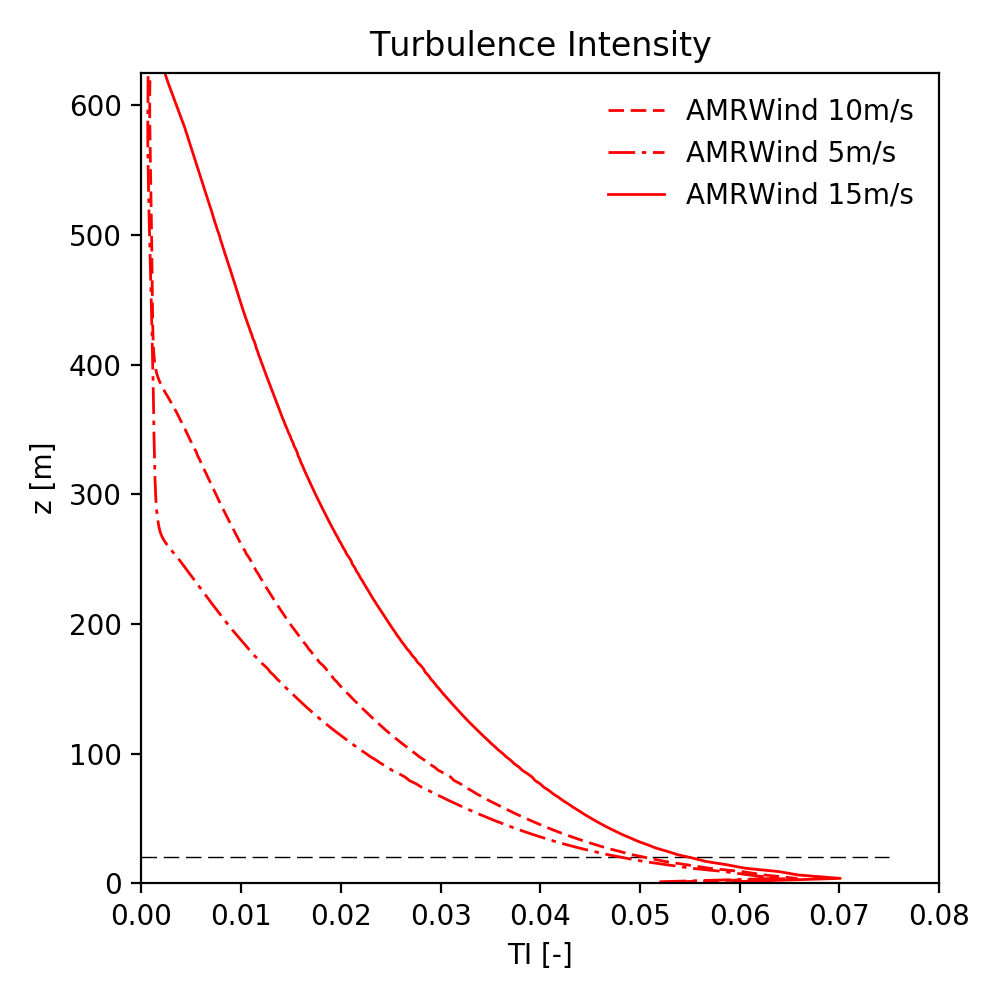
\includegraphics[width=2.5in]{figures/AMRWind_allWS/AMRWind_stable_TI.png}
  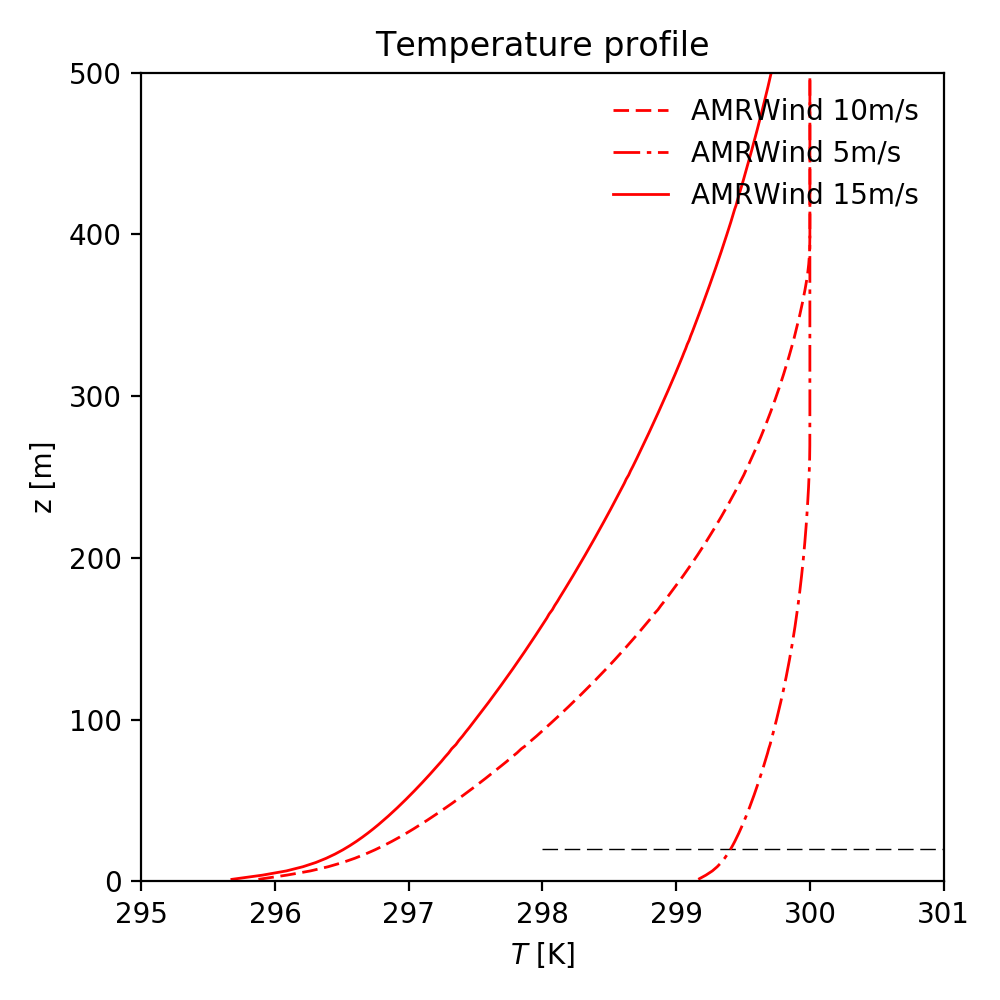
\includegraphics[width=2.5in]{figures/AMRWind_allWS/AMRWind_stable_T.png}
  \caption{ \label{fig:CompareAMRallTTI} Comparison of the turbulence
    intensity and temperature profile for the stable 5m/s, 10m/s, and
    15m/s boundary layers. }
\end{figure}
%%%%%%%%%%%%%%%%%%%%%%%%%%%%%%%%%%%%%%%%%%%%%%%%%%%%%%%%%%%%%%%%%%%%

%% \subsubsection{Wind spectra and turbulence statistics}

%% The Kaimal model for spectra \cite{kaimal1973turbulence,
%%   cheynet2017spectral} for neutral atmospheric conditions:
%% \begin{equation}
%%   \label{eq:kaimal}
%%   \frac{fS_i}{u_\tau^2} = \frac{a_i(fz/\bar{U})}{\left(1+b_i(fz/\bar{U})^{\alpha_i}\right)^{\beta_i}}
%% \end{equation}

%% %%%%%%%%%%%%%%% KAIMAL MODEL PARAMETERS %%%%%%%%%%%%%%%%%%%%%%%%%%%%%%%%%%%
%% \begin{table}[h]
%% \caption{\label{tab:KaimalParameters} Parameters for Kaimal model}
%% \centering
%% \begin{tabular}{ccccc}
%%   \hline
%%   Index $i$& $a_i$ & $b_i$ & $\alpha_i$  & $\beta_i$ \\
%%   \hline
%%   $u$      & 105.0 & 33.0  & 1           & 5/3  \\
%%   $v$      &  17.0 &  9.5  & 1           & 5/3  \\
%%   $w$      &   2.1 &  5.3  & 5/3         &   1  \\
%% \hline
%% \end{tabular}
%% \end{table}


%% %%%%%%%%%%% Stable spectra, all Z figure %%%%%%%%%%%%%%%%%%%%%%%%%
%% % Created in Postprocessing/ABLSpectra/Stable_Spectra_Allz.ipynb
%% \begin{figure}[hbt!]
%%   \label{fig:ABLSpectra_AllZ}
%%   \centering
%%   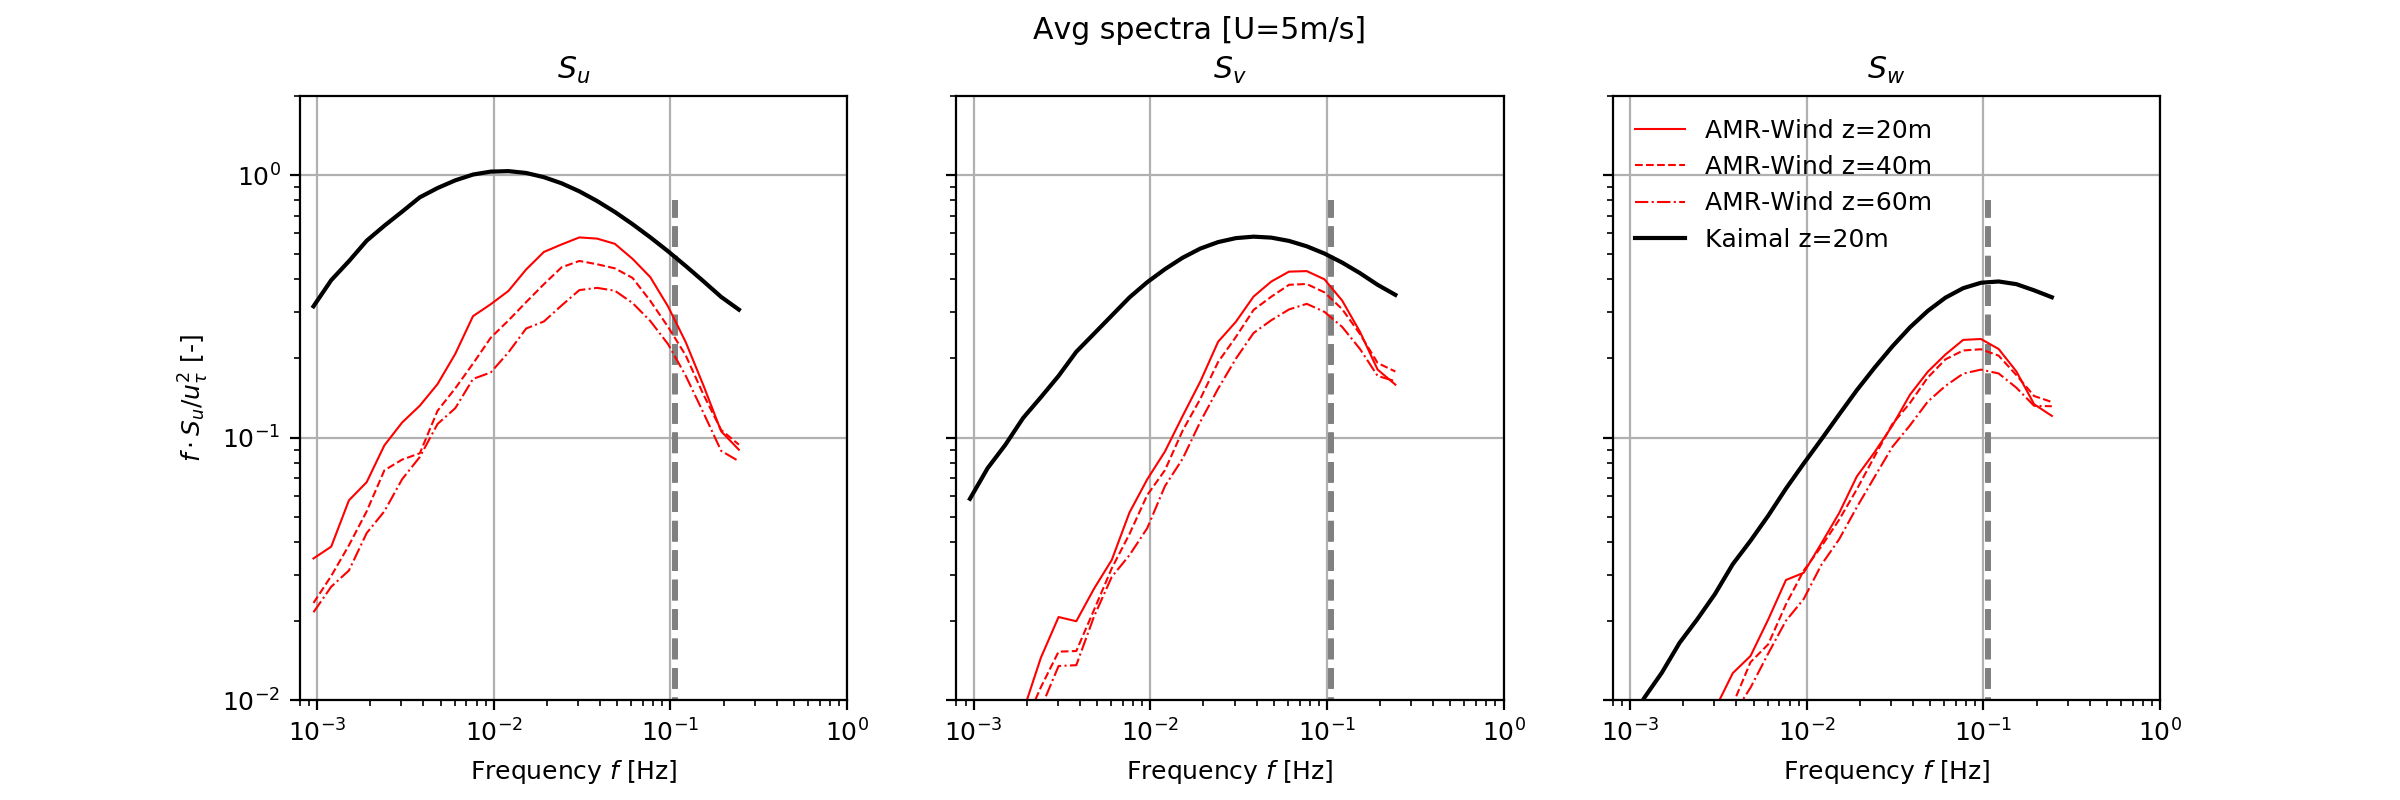
\includegraphics[width=7.0in]{figures/Stable_Spectra_AllZ_05ms.png}\\
%%   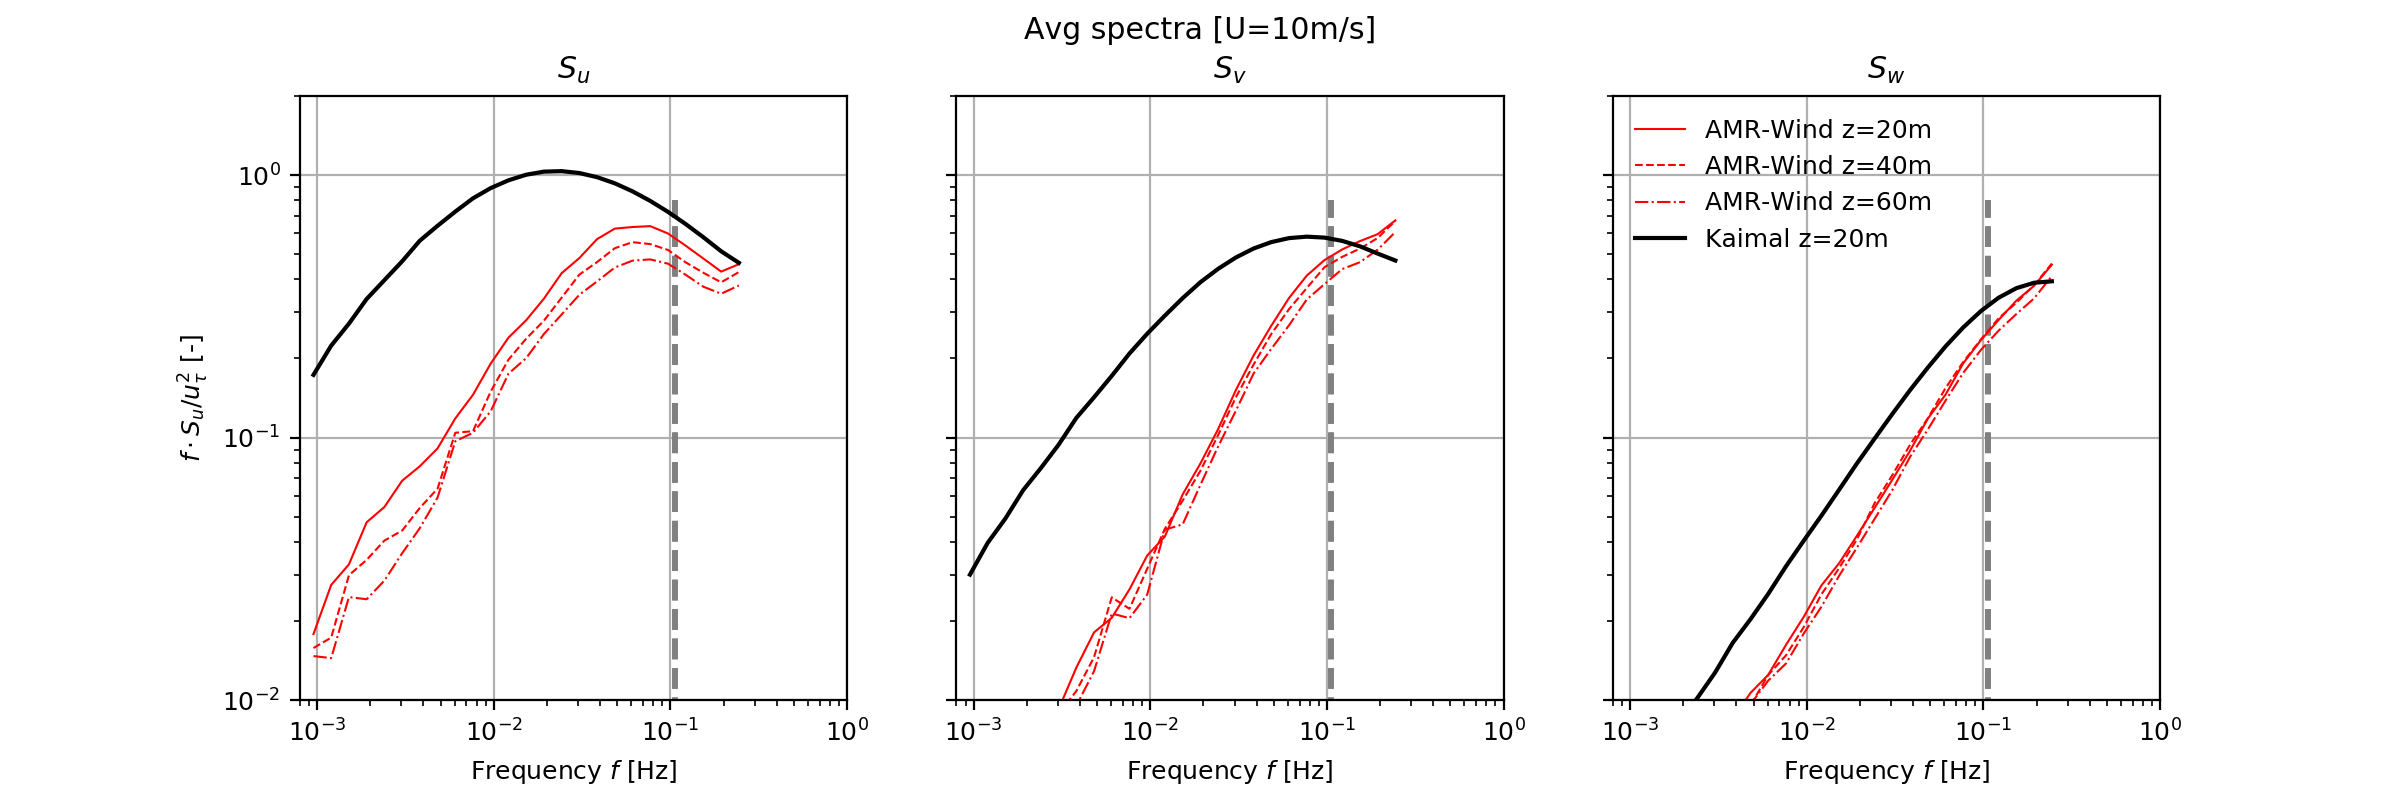
\includegraphics[width=7.0in]{figures/Stable_Spectra_AllZ_10ms.png}\\
%%   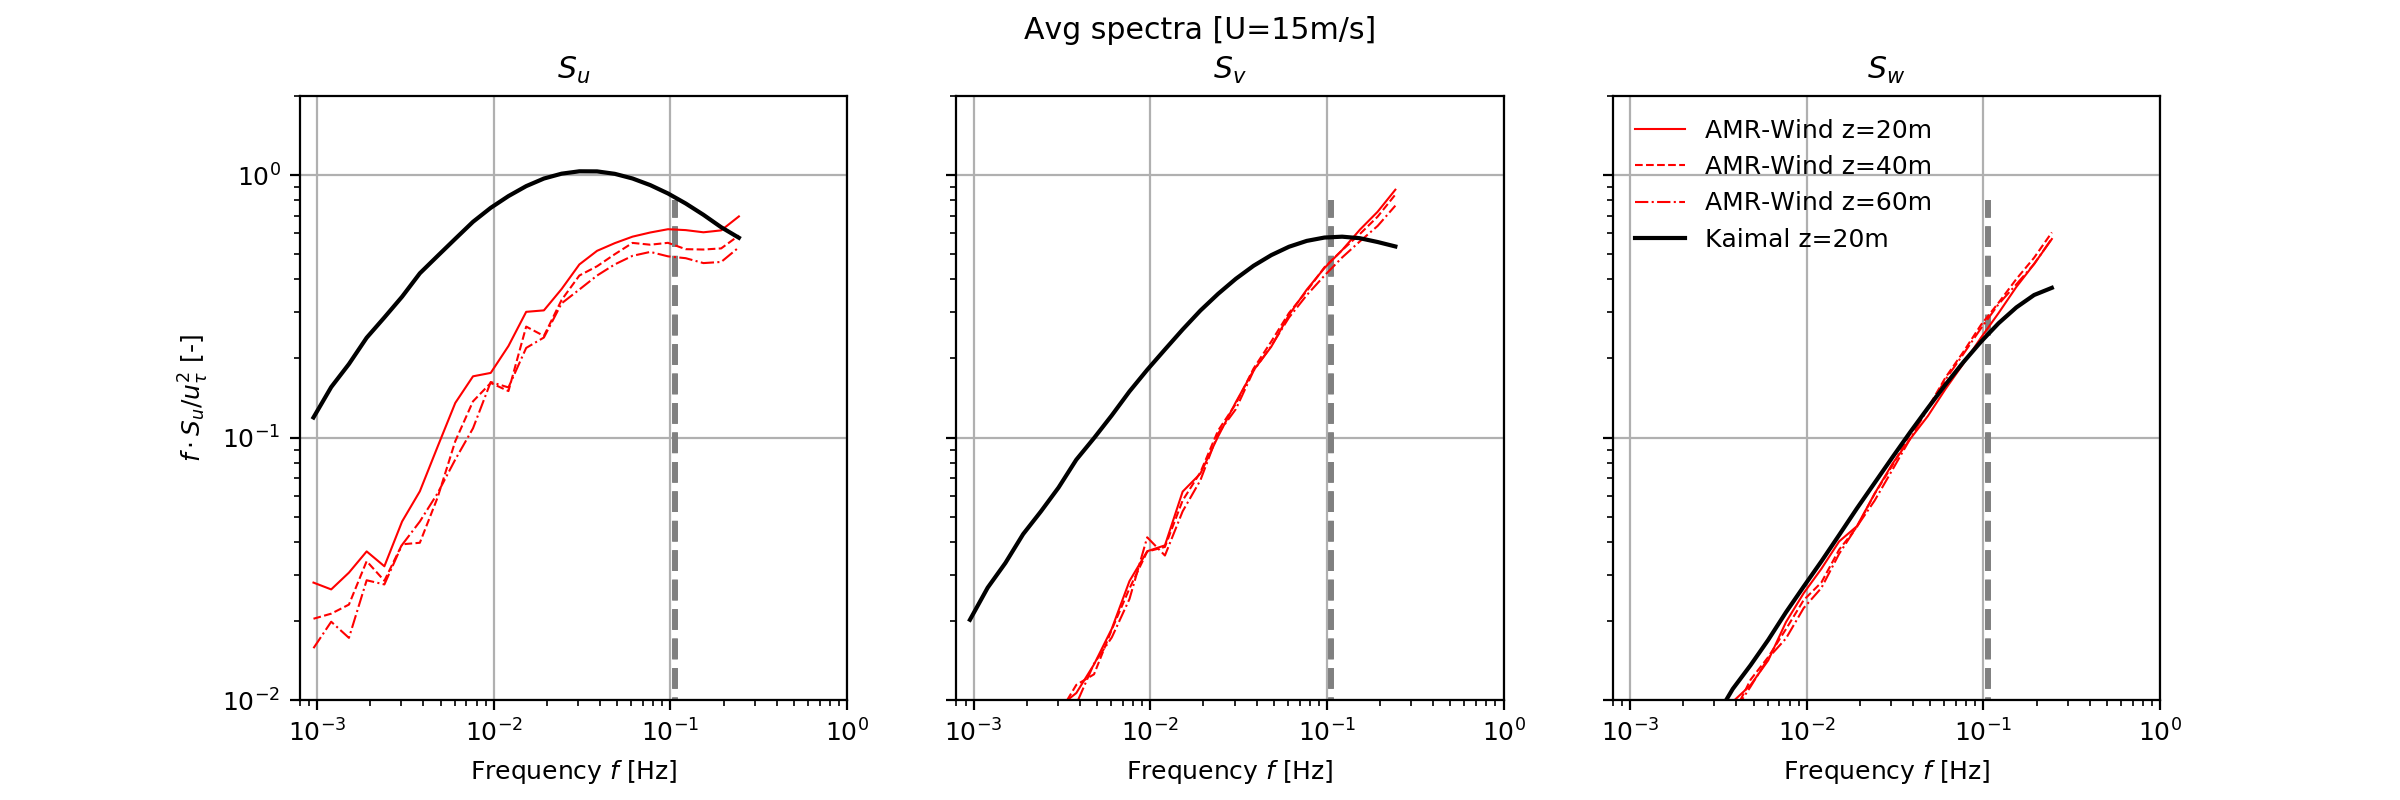
\includegraphics[width=7.0in]{figures/Stable_Spectra_AllZ_15ms.png}
%%   \caption{Calculation of the wind spectra $S_i$ for LES of stable
%%     5m/s, 10m/s, and 15m/s cases at z=20m, 40m, and 60m.  The black
%%     vertical lines correspond to the maximum resolvable frequency
%%     $f_{max}$ according to equation (\ref{eq:fmax}). }
%% \end{figure}
%% %%%%%%%%%%%%%%%%%%%%%%%%%%%%%%%%%%%%%%%%%%%%%%%%%%%%%%%%%%%%%%%%%%%%


\subsubsection{Comparison with neutral and unstable conditions}

Strong differences based on the atmospheric stratification can also be
seen when we compare the stable ABL cases with the neutral and
unstable counterparts from \cite{cheung2020large}.  In the previous
study, both neutral and unstable offshore boundary layer cases were
considered at the same 5 m/s, 10 m/s and 15 m/s wind speeds.  Similar
to the findings in \ref{sec:stableABLStats}, the 5 m/s and 10 m/s
unstable cases were classified as ``very unstable'', while the 15 m/s
was identified as ``stable'' based on the Obukhov length scale.

The impact of the stability on the turbulent structures can be seen
through the correlation statistics and calculated lengthscales in
figure \ref{fig:AllStabilityRij} and
\ref{fig:AllStabilityLengthscale}.  The large disparity between the
size of the turbulent structures in the stable and neutral or unstable
cases is immediately evident from the calculated $\langle
R_{11}(\boldsymbol{\xi})\rangle$ coefficients.  The longitudinal
lengthscales for the unstable ABL cases can also be an order of
magnitude larger than the stable ABL cases.  The large lateral
lengthscales for the very unstable ABL cases, compared to the lateral
lengthscales for the neutral and stable cases, is also worth noting.
For the 5 m/s and 10 m/s very unstable ABL cases, the lateral
dimensions of the turbulent structures are similar to the longitudinal
lengthscale.  This is consistent with the large convective structures
which develops in those cases.  For the unstable 15 m/s case, the
lateral lengthscales was closer to neutral and stable cases.  

%%%%%%%%%%% All stability correlation figure %%%%%%%%%%%%%%%%%%%%
% created in Postprocessing/ABLLength/CompareAll_ABL_Lengthscales.ipynb 
\begin{figure}[hbt!]
  \centering
  \fxnote{Fix legend and line styles} \\
  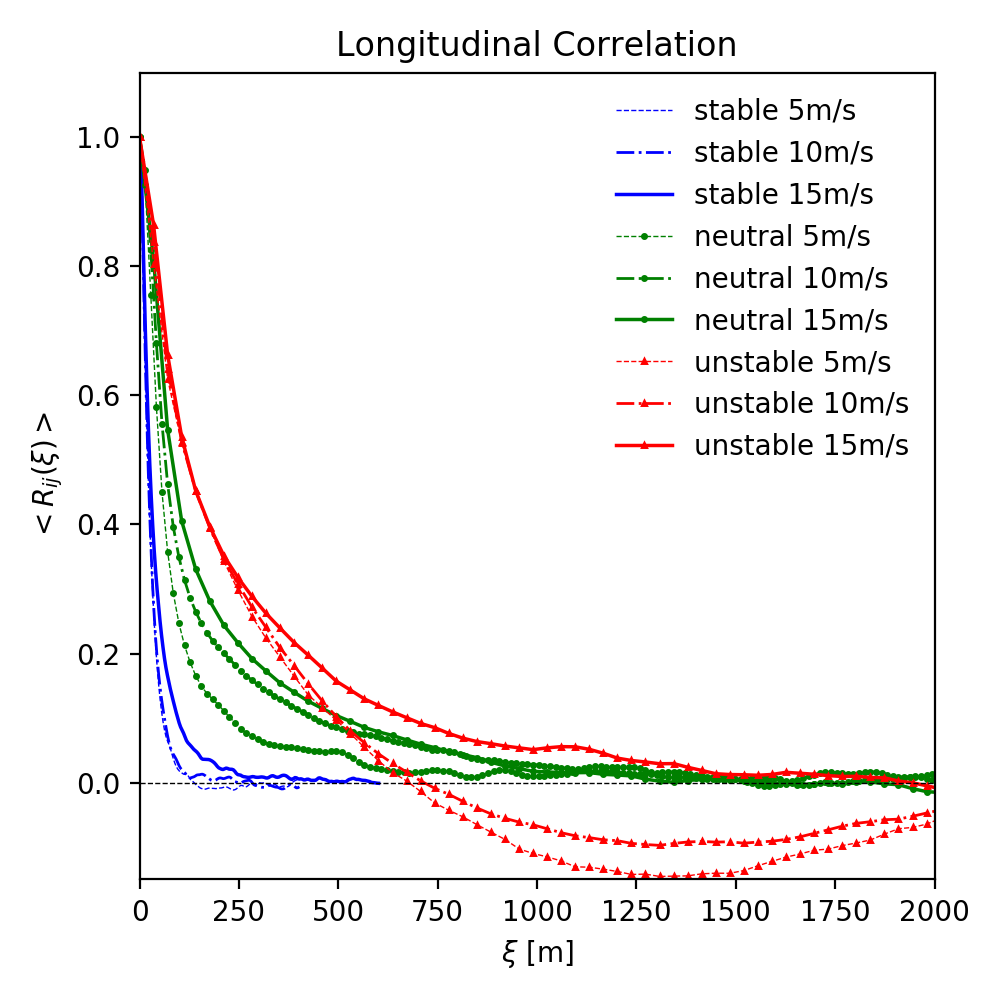
\includegraphics[width=3in]{figures/AllStability_Rij_Longitudinal.png}
  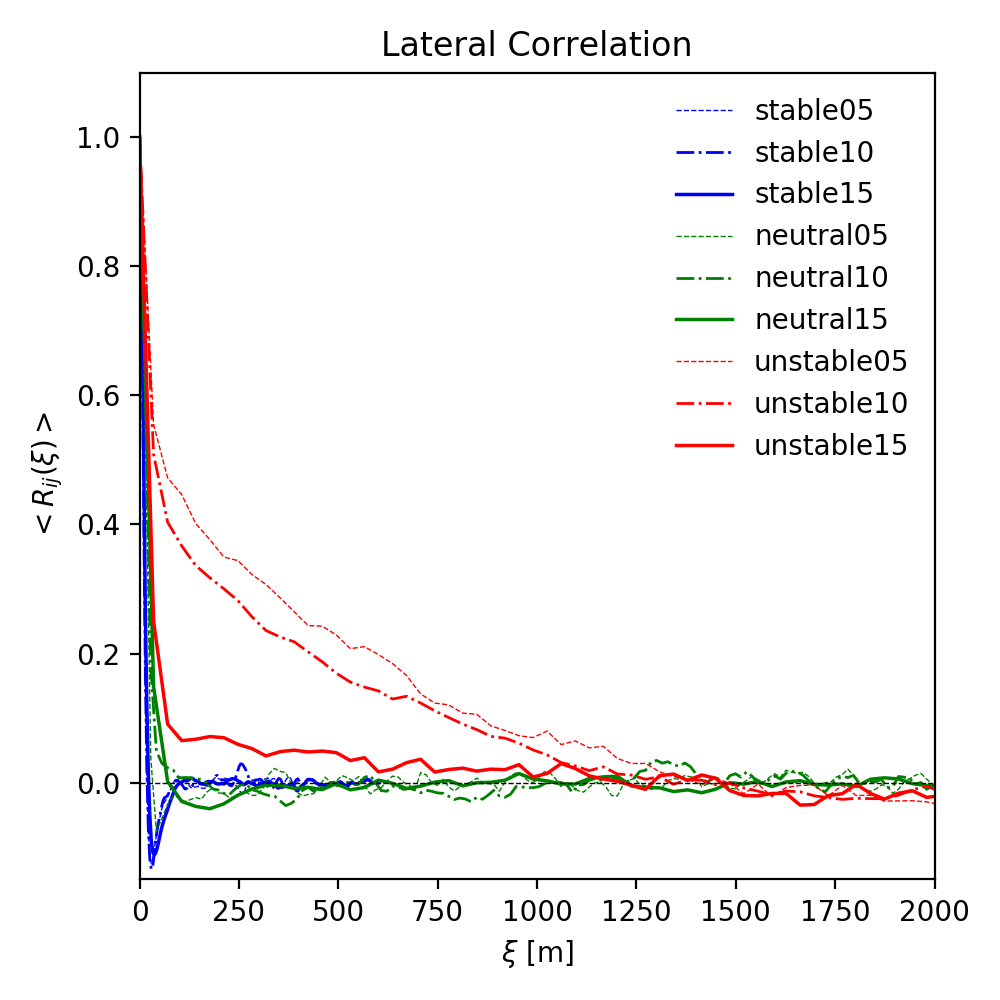
\includegraphics[width=3in]{figures/AllStability_Rij_Lateral.png}
  \caption{ \label{fig:AllStabilityRij} Calculation of the averaged
    longitudinal and lateral $\langle R_{11}(\boldsymbol{\xi})\rangle$
    coefficient at $z$=20m for all ABL stability cases.}
\end{figure}
%%%%%%%%%%%%%%%%%%%%%%%%%%%%%%%%%%%%%%%%%%%%%%%%%%%%%%%%%%%%%%%%%%%%

%%%%%%%%%%% All stability, turbulent L figure %%%%%%%%%%%%%%%%%%%%
% created in Postprocessing/ABLLength/CompareAll_ABL_Lengthscales.ipynb 
\begin{figure}[hbt!]
  \centering
  \fxnote{Fix legend and marker styles} \\
  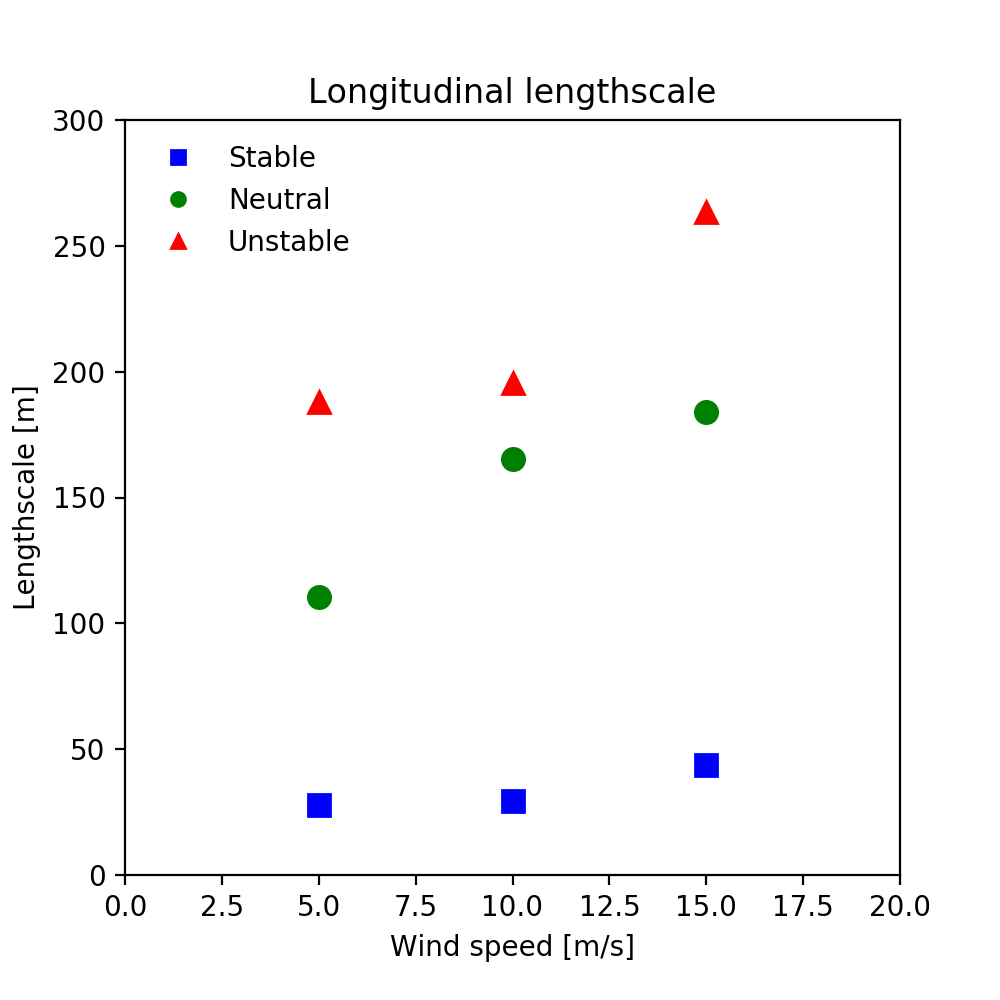
\includegraphics[width=3in]{figures/AllStability_Rij_LongitudinalLengthscale.png}
  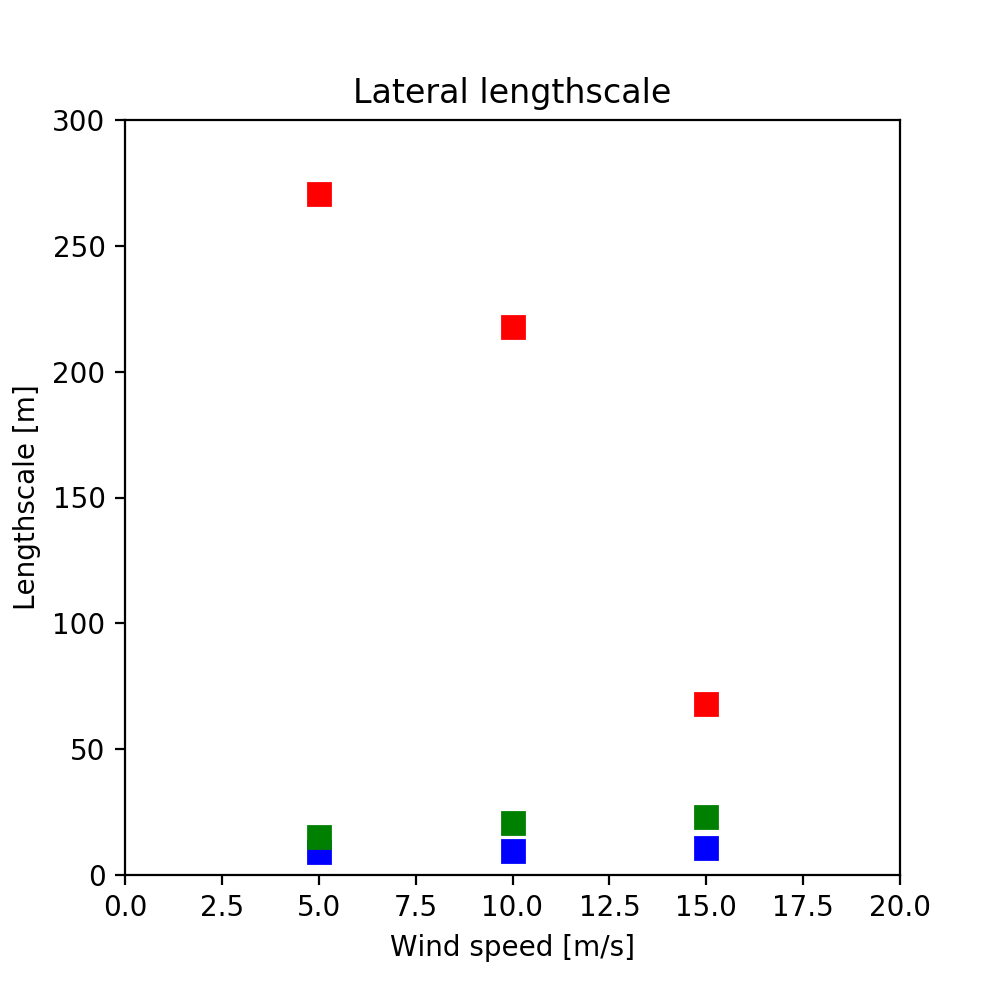
\includegraphics[width=3in]{figures/AllStability_Rij_LateralLengthscale.png}
  \caption{ \label{fig:AllStabilityLengthscale} Calculation of the
    averaged longitudinal and lateral lengthscale at $z$=20m for all
    ABL stability cases.}
\end{figure}
%%%%%%%%%%%%%%%%%%%%%%%%%%%%%%%%%%%%%%%%%%%%%%%%%%%%%%%%%%%%%%%%%%%%

%% %%%%%%%%%%%%%%% All stability: INTEGRAL LENGTH %%%%%%%%%%%%%%%%%%%%
%% % see  Postprocessing/ABLLength/CompareAll_ABL_Lengthscales.ipynb
%% \begin{table}
%% \caption{\label{tab:StabilityStudyLscale} The calculated turbulent
%%   integral lengthscale for each of atmospheric stabilities} \centering
%% \begin{tabular}{ccccc}
%%   \hline
%%   Stability   & Wind speed & Longitudinal L [m] & Lateral L [m] \\
%%   \hline
%%   Stable      &   5 m/s  & 0.0           & 0.0        \\
%%   Stable      &  10 m/s  & 0.0           & 0.0        \\
%%   Stable      &  15 m/s  & 0.0           & 0.0        \\
%%   Neutral     &   5 m/s  & 110.435741    & 15.245327  \\
%%   Neutral     &  10 m/s  & 165.398368    & 20.634052  \\
%%   Neutral     &  15 m/s  & 184.081967    & 22.961169  \\
%%   Unstable    &   5 m/s  & 187.868710    & 270.538753 \\
%%   Unstable    &  10 m/s  & 177.457502    & 215.027457 \\
%%   Unstable    &  15 m/s  & 263.475309    & 67.999898  \\
%% \hline
%% \end{tabular}
%% \end{table}
%% %%%%%%%%%%%%%%%%%%%%%%%%%%%%%%%%%%%%%%%%%%%%%%%%%%%%%%%%%%%%%%%%%%%%


\section{Conclusion}
Put conclusion here.

\section*{Appendix}

An Appendix, if needed, should appear before the acknowledgments.

\section*{Acknowledgments}

The authors wish to acknowlege the contributions from M. Churchfield
and S. Yellapantula for their development of the LES boundary
conditions and for their efforts in validating the ExaWind codes.

This research was supported by the Wind Energy Technologies Office of
the US Department of Energy Office of Energy Efficiency and Renewable
Energy.  Sandia National Laboratories is a multimission laboratory
managed and operated by National Technology \& Engineering Solutions
of Sandia, LLC, a wholly owned subsidiary of Honeywell International
Inc., for the U.S. Department of Energy's National Nuclear Security
Administration under contract DE-NA0003525. The views expressed in the
article do not necessarily represent the views of the U.S. Department
of Energy or the United States Government.

This work was authored in part by the National Renewable Energy
Laboratory, operated by Alliance for Sustainable Energy, LLC, for the
U.S. Department of Energy (DOE) under Contract No. DE-AC36-
08GO28308. M. Brazell was partially funded by the Exascale Computing
Project (17-SC-20-SC), a collaborative effort of two DOE organizations
(Office of Science and the National Nuclear Security Administration).

A portion of the research was performed using computational
resources sponsored by the Department of Energy's Office of Energy
Efficiency and Renewable Energy and located at the National Renewable
Energy Laboratory.

\bibliography{references}

\end{document}
